%% ----------------------------------------------------------------
%% Thesis.tex -- main
%% ---------------------------------------------------------------- 

\documentclass[a4paper, 10pt, oneside]{memoir}
\usepackage{basilea}

\usepackage{tikz-network}
\usetikzlibrary{patterns}
\usetikzlibrary{matrix}
\usetikzlibrary{decorations.pathreplacing}
\usepackage{amsthm}
\usepackage{wrapfig}
\usepackage{multicol}
\usepackage{amsmath}
\usepackage{tabularx}
\usepackage{pdflscape}
\usepackage{multirow}
\usepackage[inline]{enumitem}
\theoremstyle{plain}
\newtheorem{theo}{Theorem}[section]
\newtheorem{defi}{Definition}[section]
\newtheorem{assu}{Assumption}[section]
\newtheorem{prop}{Proposition}[section]
\newtheorem{remark}{Remark}[section]
\newtheorem{note}{Note}[section]
\newtheorem{cor}{Corollary}[section]
\newtheorem{ques}{Questions}[section]
\newtheorem{lem}{Lemma}[section]
\newcommand{\parenv}[1]{\left( {#1} \right)}
\newcommand{\ceilenv}[1]{\left\lceil {#1} \right\rceil}
\newcommand{\mathset}[1]{\left\{ {#1} \right\}}
\newcommand{\sparenv}[1]{\left[ {#1} \right]}
\newcommand{\Prob}[1]{\mathbb{P}\!\left[{#1} \right]}
\newcommand{\Ex}[1]{\mathbb{E}\!\left[{#1} \right]}
\newcommand{\Var}[1]{\mathbb{E}\!\left[({#1} -\Ex{#1})^2 \right]}
\newcommand{\personComment}[2]{{\noindent\color{teal}[\underline{#1:} #2]}}
\newcommand{\ludovic}[1]{\personComment{Ludovic}{#1}}
\newcommand{\ap}[1]{\personComment{AP}{#1}}
\newcommand{\alexandre}[1]{\personComment{Alex}{#1}}
\newcommand{\td}{\tilde{d}}
\newcommand{\eqdef}{\triangleq}
\renewcommand{\arraystretch}{1.3}
\setcounter{tocdepth}{3}
\setcounter{secnumdepth}{3}
%% ----------------------------------------------------------------
\begin{document}

\selectlanguage{english}

\thesisfront
\maketitle
\pagestyle{thesis}


%% ----------------------------------------------------------------
\chapter{Acknowledgments}
In the first place, I wish to thank Ludovic Barman and Apostolos Pyrgelis for making this master project possible, but also for their precious advice, support and good mood all along my master project. I would also like to thank Jonathan Guisolan, Cedric Dumur and Charles Gallay for reading this thesis and their feedback. Finally, I wish to thank my family for always encouraging me and supporting me all along my studies.
%% ----------------------------------------------------------------
\chapter{Abstract}
Smartwatches store, process, and communicate a lot of personal and sensitive information (notably related to the owner's lifestyle and health). In this thesis, we explore the feasibility of inferring sensitive information from encrypted Bluetooth traffic between a smartwatch and its paired smartphone. We consider a passive eavesdropper monitoring the encrypted Bluetooth transmissions, without breaking the Bluetooth encryption scheme nor interacting with the devices, and we show that such attacker can infer sensitive information such as the application currently running and actions performed by the user. To carry out the attack, we first build a system that generates data at large scale by automating actions on the smartwatches. Then, we design a Machine-Learning based model that infers application usage on smartwatches. We analyze relevant features for application and action identification, and find out that packet inter-arrival-time, sizes and directions reveal enough information for the attack to be successful. We show how our model generalizes between smartwatches of different vendors, and how it can be used to perform long-term activity tracking (over the course of a day).

%% ----------------------------------------------------------------
\thesistoc

%% ----------------------------------------------------------------
%\thesisnomencl
%% ----------------------------------------------------------------
\thesismain

\chapter{Introduction}
\label{chap:Introduction}
Smartwatches are small computing devices that are worn as traditional watches. They have a lot of capabilities and can perform almost all operations that a smartphone can do such as making phone calls, sending messages, retrieving emails. But the real asset of smartwatches comes from their ability to provide more advanced services, helping users to manage their smoking habits, remember their medication or monitor their heart rate. 
\\
\\
One important feature of smartwatches is their ability to be personalized by their owner. Every smartwatch has access to an application store (e.g.  Google Play store, App Store) where the user can download any application that is suitable for his usage. Many types of applications exist, ranging from medical, religious or news applications.
\\
\\
Nevertheless, the presence of these applications carry personal information that could enable profiling. Applications running on smartwatches often exchange information with their paired smartphone via Bluetooth. Due to the broadcast nature of Bluetooth, nothing prevents a local attacker to passively record the encrypted Bluetooth traffic of smartwatches to infer sensitive information about the watch's owner.


\section{Motivation}

Knowing which applications are installed on a smartwatch can reveal sensitive information and could hurt individual’s interests for the benefits of the attacker. We illustrate this claim by giving few scenarios in which such information can be turned against the victim's interest. 


\begin{itemize}
	\item Health Insurance tracking particular apps to decide health coverage.\footnote{\url{https://www.theglobeandmail.com/technology/how-insurers-are-turning-to-fitness-apps-to-decide-your-health-coverage/article16065068/}} Tracking, for instance, diabetes manager apps to increase insurance rate of individuals.
	
	\item Governments tracking individuals having particular religious application to increase their surveillance level.\footnote{\url{https://www.pewresearch.org/fact-tank/2016/06/28/religious-restrictions-among-the-worlds-most-populous-countries-2/}}

	\item Universities, Schools overhearing traffic to fight against cheaters that use translate software on their smartwatch.\footnote{\url{https://www.irishtimes.com/news/education/smartwatches-linked-to-spike-in-college-exam-cheating-1.3978932}}
	\item Advertiser targeting specific applications. For instance, fitness applications for an advertising campaign on protein supplement powder, or a particular news app that leaks political views.
\end{itemize}

\newpage

These examples indicate that the reason for such an attack are multiple and diverse, and the attacker himself can take many forms: a noisy neighbor, an advertiser in a mall, or governments. Therefore, we believe that understanding \emph{how well} such attacks perform would be a valuable contribution.
\\

In addition to the obvious privacy threat, we note that an attacker aware of a vulnerability in a specific application would be able to track this application without having to scan each smartwatch to exploit the vulnerability.


\section{Problem statement}
This Master Thesis aims to answer the following question:

\begin{quote}
Is it feasible for a passive attacker to infer information by recording encrypted Bluetooth traffic between a smartwatch and its paired mobile phone?    
\end{quote}

More specifically, we will investigate if an attacker can fingerprint an application and its usage from its generated encrypted traffic within a specific set of applications.  \\

To answer the above question, we will go through the following points which represent our contribution:

\begin{itemize}
	\item Identify and select what kind of personal information an attacker can infer from encrypted Bluetooth traffic between a smartwatch and a smartphone.
	\item Construct an automated system that allows data collection at scale.
	\item Propose and evaluate an attack that infers installed applications and actions from encrypted Bluetooth traffic between different smartwatch-smartphone pairs.
	\item Discuss and investigate how generic and realistic the attack is.
\end{itemize}




\section{Thesis structure}
The structure of this thesis goes as follows: \\

In Chapter~\ref{chap:Background}, we provide background knowledge. In Chapter~\ref{chap:related_work}, we explore the related work. In Chapter \ref{chap:attack overview}, we give an overview of the attack along with our threat model. In Chapter~\ref{chap:methodology}, we explain the methodology we follow to construct the attack. In Chapter \ref{chap:Generalization}, we explore how generic is the attack. In Chapter \ref{chap:towards_a_realistic_attack}, we discuss how realistic is the attack. Finally, in Chapter \ref{chap:Conclusion}, we draw Conclusion of our research and discuss some future works.
\chapter{Background}
\label{chap:Background}
In this chapter, we provide background knowledge about Smartwatches and Bluetooth as well as Random Forest and Evaluation metrics.


\section{Smartwatches}
\label{sec:smartwatches}
There exist many brands of smartwatches running multiple operating systems. \textit{WearOS}, \textit{WatchOS} and \textit{Tizen} are amongst the main actors. WatchOS and Tizen are dedicated to run principally on Apple Watch and Samsung watches respectively; whereas WearOS is run by many different brand such as Huawei, Fossil, Motorola or even Louis Vuitton. In this thesis, we focus on three different smartwatch brands: \textbf{Huawei}, \textbf{Fossil} and \textbf{Apple}, which represents more than 40\% of the market share as of 2019. Fig.~\ref{fig:marketshare smartwatches.jpg} shows the market share of smartwatches by brands.


\begin{figure}[H]
 \centering
 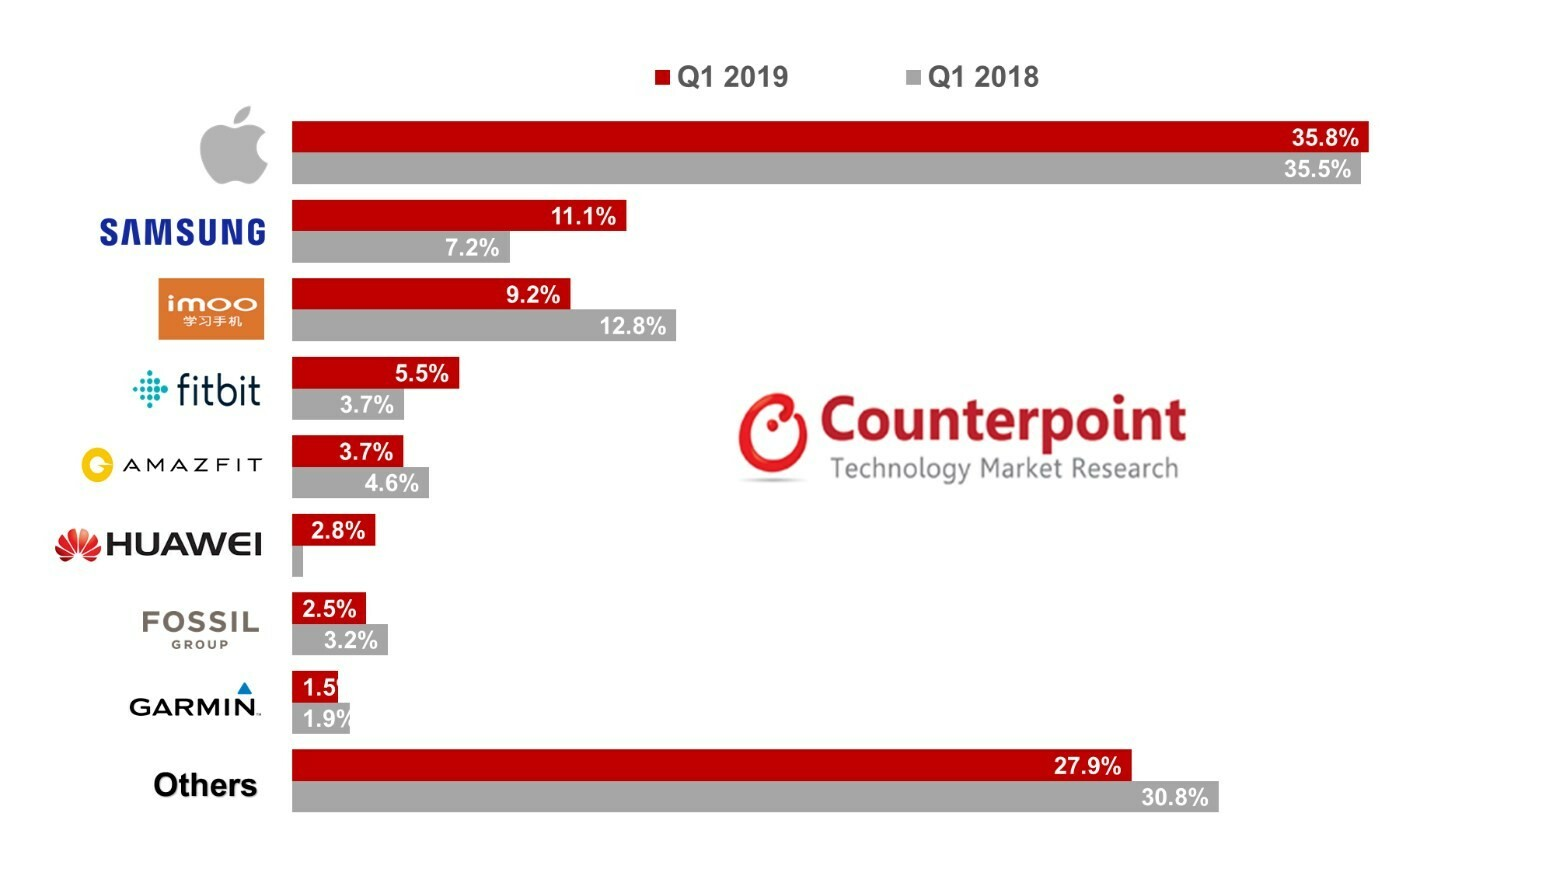
\includegraphics[width=0.9\textwidth]{figures/marketshare smartwatches.jpg}
 \caption[test]{Market share of smartwatches by brand in 2018 and 2019.\footnotemark}
 \label{fig:marketshare smartwatches.jpg}
\end{figure}
\footnotetext{Picture taken from https://www.notebookcheck.net/Latest-report-shows-1-in-every-3-smartwatches-sold-in-2019-so-far-was-an-Apple-Watch.420045.0.html}




\paragraph{Connectivity.} Most smartwatches are equipped with both Wi-Fi and Bluetooth interfaces. Even though Wi-Fi is supposed to provide a better throughput to access the Internet, a study shows that Bluetooth traffic is responsible for more than 91\% of the total traffic~\cite{10.1145/3081333.3081351}. The main reason is to save energy, since Bluetooth consumes less than Wi-Fi. Many possible events can be at the origin of data transfer over Bluetooth: push notifications\footnote{\textbf{Push notifications} are piece of information possibly coming from the outside world to notify the user of a particular event}, background updates or more naturally the user's interaction with the smartwatch.

\paragraph{Application Store.} Most smartwatches allow anyone to develop and deploy applications on their application store. However, it has to be noted that application stores of smartwatches are much more constrained than smartphone's application stores. In fact, smartwatches stores are more focused on Health, Fitness and Reminders applications; games for instance are almost non-existent due to the small screen size of smartwatches. 


\section{Bluetooth}
\label{sec:Bluetooth}
Bluetooth is a full stack protocol which is widely used to create Wireless Personal Area Network (WPAN). Nowadays, most personal mobile devices are equipped with Bluetooth interfaces. In that manner, the Bluetooth Special Interest Group (SIG) reported an expected increase from 0.9 billion annual unit shipment in 2020 to 1.5 billion in 2024 for data transfer devices such as smartwatches \cite{bluetoothMarket}. In this section we explain only relevant background about Bluetooth and we refer the reader to the Bluetooth Core specifications for further technical details \cite{bluetoothSpecs}.



\paragraph{Bluetooth Classic and Low Energy.} Two types of Bluetooth operate: Bluetooth Classic (Also known as BR/EDR) and Bluetooth Low Energy (BLE). Bluetooth Classic is intended for communication with intensive data transfer, while BLE aims to provide a communication that is energy efficient. Since most smartwatches are using Bluetooth Classic only, we will simply use Bluetooth to refer to Bluetooth Classic. 


\paragraph{Frequency-Hopping Spread Spectrum.} Bluetooth uses frequency-hopping spread spectrum (FHSS). It consists of dividing the allocated spectrum into narrow band subchannels and the time into slots of 625ns duration. In each time slot, a designated frequency band is used to transmit the signal. The frequency-hopping sequence is pseudo randomly generated and is derived by the peers taking part in the communication before the actual data transfer begins. When Bluetooth senses too much interference on a particular frequency band, it performs adaptive hopping which will bane the usage of this band of a period of time.  


\paragraph{Eavesdropping Bluetooth traffic.} Because of the FHSS scheme, it has long been considered technically difficult to eavesdrop Bluetooth communications. However, due to hardware improvements, many devices with Bluetooth eavesdropping capabilities start emerging. The cost and the efficiency of these devices vary a lot. Devices such as Ellisys Vanguard\footnote{Throughout this thesis, we use this device to record Bluetooth traffic. \url{https://www.ellisys.com/products/bv1/index.php}} can concurrently overhear multiple communications by listen on all subchannels in parallel; providing a perfect capture rate, but at a considerable cost. However, Albazrqaoe et al. designed a system that can overhear a targeted Bluetooth communication at a capture rate of more than 90\% with two Ubertooth costing 80\$ per unit~\cite{blueEar}. 

\paragraph{Communication range.} Since Bluetooth signals operate at a high frequency of 2.45 GHz, it is designed for short-range communication of around 10 to 200 meters depending on the Bluetooth version and the environment. However by boosting the Bluetooth's receiver antenna, one can increase greatly the range of sniffing Bluetooth traffic. This might be particularly helpful for an attacker being a bit further from his victim.

\newpage

\paragraph{Security.} There are four security levels in Bluetooth. In level 1, no encryption is required. This level is typically used for advertising purposes. Level 2 uses AES-CMAC encryption for unpaired communication~\cite{rfc4493}. Level 3 is the same as level 2 with pairing required. Level 4 requires pairing and Elliptic Curve encryption, namely ECDHE~\cite{hankerson2006guide}. In Bluetooth Classic,  most data transfer is done with security level 3 or 4 which makes the decryption difficult. Thus, if pairing is done correctly, payloads are confidential, but not metadata such as the Bluetooth MAC address which is still sent in cleartext. In addition to encryption, MAC address randomization can be deployed to enhance privacy. In Bluetooth Classic, it consists to change frequently the three most significant bytes of the Bluetooth address. However, an attacker can still track specific traffic by looking at the three least significant bytes of the Bluetooth address which are invariant over time.



\section{Random Forest}
\label{sec:RF}
We use Random Forest (RF) to build our attack. RF is a supervised Machine Learning model which is widely used for data classification tasks~\cite{breiman2001random}. It is an Ensemble method which means that the classifier is composed by many weak learners called decision trees (or estimators). The output prediction will be averaged over all the decision trees predictions in the Random Forest.  \\ 

In the Random Forest, each decision tree is grown on an independent subset of features and samples with the following procedure: Make branches by splitting recursively the data according to their most discriminant feature. Once all samples belong to the same class, create a leaf that belongs to that class. If no features are left for splitting, create a leaf and assign the class to the majority. To make a prediction, simply flow down the tree until reaching a leaf. Fig.~\ref{fig:random_forest} shows the decision process of a Random Forest using majority voting. 

\begin{figure}[H]
 \centering
 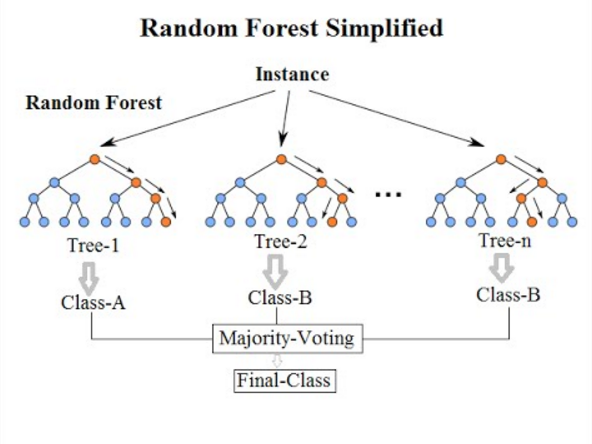
\includegraphics[width=0.6\textwidth]{figures/random-forest.png}
 \caption[test]{Decision process of a Random Forest using majority voting\footnotemark}
 \label{fig:random_forest}
\end{figure}
\footnotetext{Picture taken from https://miro.medium.com/max/1184/1*i0o8mjFfCn-uD79-F1Cqkw.png}



\newpage


\section{Evaluation Metrics}
\label{sec:background evaluation}
The evaluation metric reflects how the model performs. Picking a good evaluation metric is therefore an important step. We will use different evaluation metrics throughout this thesis:

\paragraph{Accuracy.} Accuracy is probably the mostly used and intuitive evaluation metric. It is computed as the total number of correct predicted samples over the total number of samples. It can be computed over all classes or be specific to one class. It gives a taste of what fraction of time we are making good prediction.

\\



 \paragraph{Precision and Recall.} 

Accuracy, is sometime not enough to evaluate a model. To gain more insight, we will also use precision and recall. Before explaining what precision and recall is, we will have to defined the following quantities:

\begin{itemize}
    \item \textbf{True Positive (TP):} Number of samples belonging to a particular class \textbf{correctly} predicted to belong to this class.
    
    \item \textbf{True Negative (TN):} Number of samples \textbf{not} belonging to a particular class \textbf{correctly} predicted to \textbf{not} belong to this class.

    \item \textbf{False Positive (FP):} Number of samples \textbf{not} belonging to a particular class \textbf{wrongly} predicted to belong to this class.

    \item \textbf{False Negative (FN):} Number of samples belonging to a particular class \textbf{wrongly} predicted to \textbf{not} belong to this class.
\end{itemize}

Precision and recall can then be computed with the following formulas:
\begin{itemize}
    \item $Precision=\frac{TP}{TP + FP}$
    \item $Recall = \frac{TP}{TP + FN}$
\end{itemize}

Precision represents the fraction of time we are correct about a class when predicting this class. Whereas recall represents the ability of detecting a certain class when that class appears. These metrics are particularly useful to evaluate the performance of a particular class. We would expect an attacker targeting fitness apps to find the best spot for its advertising campaign, to privilege a good recall score on fitness apps than a good precision score. On the opposite, we would expect an attacker targeting students cheating with their smartwatch to privilege a good precision score. 



\paragraph{F-beta score.} The F-beta score is a mixture of precision and recall. It is computed as the weighted harmonic mean between recall and precision. When the weight beta is equal to 1 we are talking about F1 score which means that we are caring equally much about precision than recall. The F-beta score is computed as follows:


$$ F_\beta = (1 + \beta^2) \cdot \frac{\mathrm{precision} \cdot \mathrm{recall}}{(\beta^2 \cdot \mathrm{precision}) + \mathrm{recall}}$$


\paragraph{Confusion Matrix.} Confusion Matrix are useful representations that assess the performance of a classifier. In our case, each raw of the matrix represents the normalized number of true instances belonging to a particular class while each column represents the predicted instances belonging to a particular class. The diagonal of the matrix represents the normalized number of correct classified predictions.




\paragraph{Cross-validation.}

Cross-validation is a technique used to evaluate a model which provides better confidence about the performance. It consists of splitting train and test data multiple times differently. This ensures that not always the same data are used as train and test. There exists multiple variations of cross-validation. In our case we will use n-Random-Split cross-validation which consists of splitting train and test data randomly n times.
\chapter{Related Work}
\label{chap:related_work}
This Chapter explores the related work on encrypted traffic-analysis attacks in various contexts. We separate traffic-analysis attacks into 3 categories \textit{Website Fingerprinting}, \textit{Mobile Application Fingerprinting} and \textit{Wearable Devices Fingerprinting}.

\paragraph{Website Fingerprinting (WF).} WF consists of identifying web pages from their encrypted traffic traces. WF has been broadly studied under diverse assumptions. Early work on WF started in 1998 on HTTP 1.0 over SSL by leveraging HTTP objects count and sizes~\cite{cheng1998traffic, 10.5555/829514.830535}.  Later on, with HTTP 1.1, persistent connection was used making resources isolation not possible. In 2006, Levine et al. proposed an attack over 2,000 web pages only based on packet sizes discarding the assumption of isolating resources~\cite{liberatore2006inferring}. In 2011, Panchenko et al. constrained the assumption of observable packet length by constructing an attack on the Tor web browser~\cite{10.1145/2046556.2046570}. After that, many researchers further improved the results from Panchenko et al. on Tor by considering different models \cite{cai2012touching, 10.1145/2517840.2517851, 184463}. In 2016, Wang et al. investigated an attack under various more realistic conditions such as an attacker who does not know when traffic of web pages starts and ends \cite{OnRealisticallyAttackingTorwithWebsiteFingerprinting}. In a concurrent work, Hayes et al. provided a new WF attack by using an adapted version of RF to generate fingerprint. In their work, they identified 30 monitored web pages out of 100,000 unmonitored web pages which pushed away the closed-world assumption where the victim is only visiting a constrained number of web pages~\cite{k-fingerprinting}. Nowadays, the state-of-the-art WF on Tor are based on Convolutionnal and Deep Neural Network model, archiving around 98\% to 99\% accuracy~\cite{he2018deep, bhat2019var, rahman2019tik}. 



\paragraph{Mobile Application Fingerprinting (MAF).} With the increase in popularity of smartphones, researchers also studied MAF.  Which consists of fingerprinting mobile applications and actions from the traffic they generate. Perhaps the first work to target multiple mobile applications was due to Conti et al. in 2015~\cite{conti2015can}. In their work, they fingerprinted 17 actions from across different applications. Later on, they extended their first paper to provide an attack that works on seven different applications and multiple actions per application~\cite{conti2015analyzing}. Then, researchers improved their results in terms of number of application fingerprinted. In this way, a system called Appscanner, with automatic dataset generation capabilities using \texttt{adb} and \texttt{monkeyrunner}\footnote{We also used adb and monkeyrunner for our automation system. However, our system is significantly different, as it works on smartwatches and we collect traces over Bluetooth.} could successfully fingerprint up to 110 applications using Random Forest~\cite{taylor2016appscanner}. However, criticizes emerged as their system was not robust over time and across different OS versions~\cite{taylor2017robust}. More recently, Wang et al. proposed an automation tool to generate the dataset from real 28 users over two periods of 4 and 10 weeks. They achieved 91.8\% accuracy on a 1D CNN classifier over 142 application~\cite{wang2020real}.

\newpage


\paragraph{IoT Devices Fingerprinting (IDF).} Das et al. inferred fitness tracker devices over Bluetooth LE, by listening on advertising channels~\cite{das2016uncovering}. In their paper, they also classified four types of physical activities amongst 10 persons from encrypted BLE traffic. Acar et al. achieved 90\% accuracy on fingerprinting diverse IoT devices and their respective state/activity on BLE and two other protocol~\cite{acar2018peek}. Aksu et al. identifies models of smartwatches devices using Inter-Arrival-Time (IAT) of Bluetooth packet~\cite{fingerprintWearableDevices}. However, their approach implies a Bluetooth sniffer directly inside the smartphone. Our attack uses a Bluetooth Recorder external to the smartphone.  





\paragraph{Differentiation from previous works.} Our work has several important differences compared to the aforementioned works. First and foremost, WF and MAF both performs traffic-analysis on top of TCP/IP packets, hence the network stack is fairly different. WF targets web pages, for which it is much easier to build large dataset. Moreover, compared to WF, there is no mechanism such as Tor that hides packet length, thus our attack can fully exploit features based on packet length. While MAF also targets applications, the work presented take advantages of particularities in TCP/IP that we cannot exploit with Bluetooth (such as TCP re-transmission flags or IP destination address). Fingerprinting wearables is a relatively new field, and while BLE showed obvious privacy leakage on advertising channels, our work focus on Bluetooth Classic. Finally, none of the work we presented was intended to target smartwatch applications over Bluetooth. 




\chapter{Attack Overview}
\label{chap:attack overview}
In this chapter, we first describe the attack and then specify the assumptions we make about the victim and the attacker.

\section{Attack Flow} First, a user preforms an action\footnote{\textbf{Action} is defined as a sequence of instruction related to a specific application to achieve a goal. Example: \texttt{addInsulin} is one possible action in the application DiabetesM. We consider that \texttt{opening} and \texttt{closing} applications are actions as well.} related to a targeted application on her smartwatch. This action triggers an encrypted Bluetooth communication between the smartwatch and its paired mobile phone. All this communication is captured by a local attacker. Finally, the attacker guesses which application generated the encrypted capture. Fig. \ref{fig:attack_overview} illustrates an overview of the attack.


\begin{figure}[H]
 \centering
 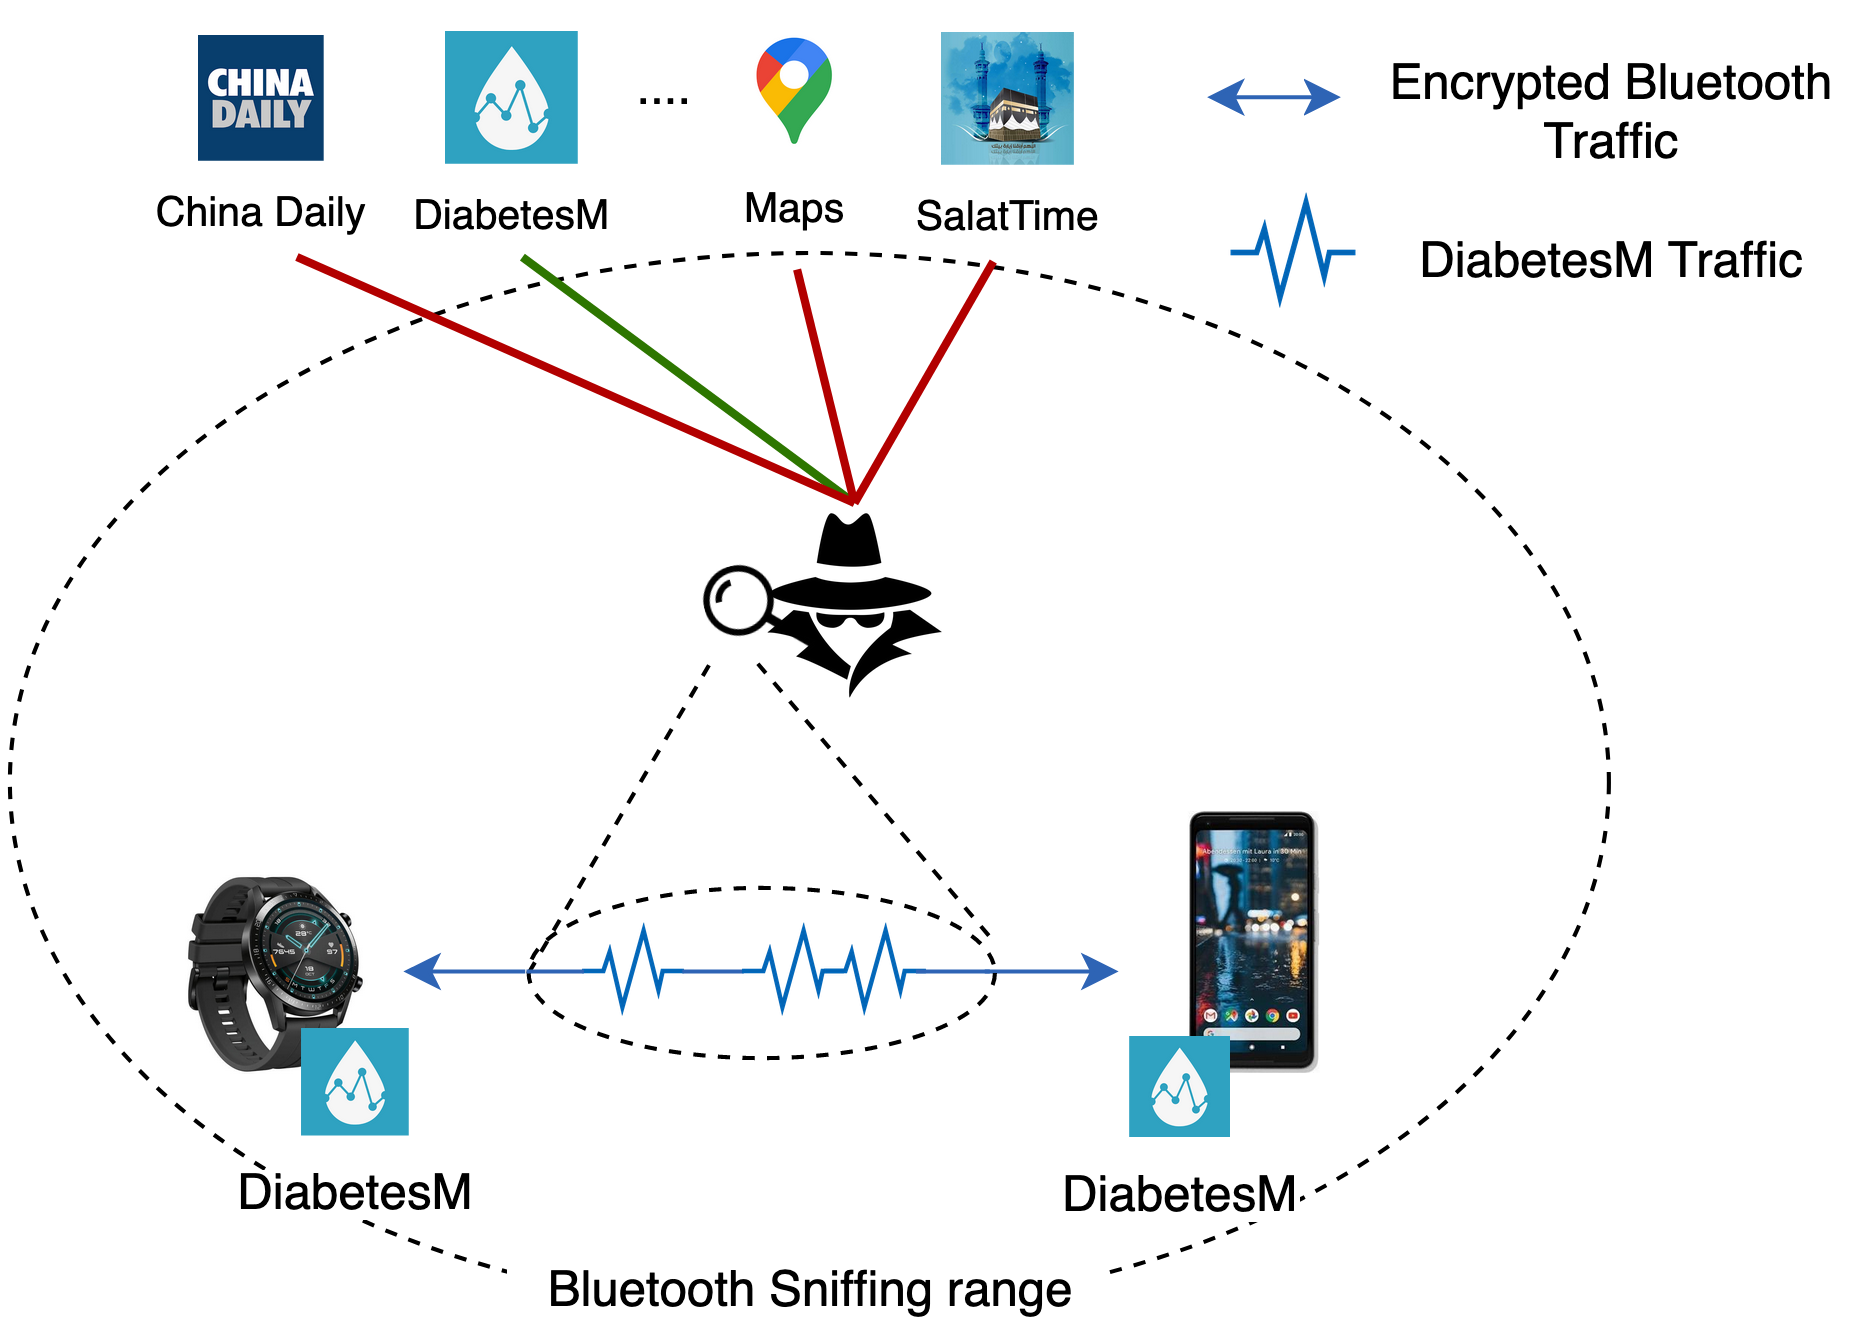
\includegraphics[width=0.8\textwidth]{figures/attack_overview.png}
 \caption[test]{Attack overview. An attacker is guessing correctly that the encrypted traffic recorded is from the Application DiabetesM\footnotemark}
 \label{fig:attack_overview}
\end{figure}
\footnotetext{\textbf{DiabetesM} is an application that helps diabetics to manage their diabetes.}


In Fig~\ref{fig:attack_overview}, the attacker is represented by a physical person. This can be the case if an attacker specifically follows a person to capture its Bluetooth traces with a portable sniffing device. However, we would more expect the attacker installing one or more sniffing devices at some location and coming from time to time to collect Bluetooth traces or directly transferring these traces to a remote server for a real-time analysis. 


\section{Threat Model} To summarize, we make the following assumptions regarding the attacker: 


\begin{enumerate}

    \item \textbf{Proximity}: The attacker is local to the victim.
    
    \item \textbf{The attacker is able to monitor the traffic}: The attacker possess the technology to monitor a targeted Bluetooth traffic.
    
    \item \textbf{Closed-World}: The victim is only using applications within a constrained set of applications which is known by the attacker.
    
    \item \textbf{Single-Action Capture}: The capture processed by the attacker contains only traffic related to a single action performed on the smartwatch.
    
    \item \textbf{Passive Attacker}: The attacker does not alter in anyway the communication between the victim's smartwatch and smartphone.
    
    \item \textbf{External Attacker} The attacker has no access to victim's phone or smartwatch. However, we assume that he has access to similar types of devices that he can buy.
    
    \item \textbf{The attacker cannot decrypt the traffic content}: We consider that the attacker is not able to decode the traffic. He deals only with encrypted traffic to infer information.
    
\end{enumerate}
\\
We saw in Sec.~\ref{sec:Bluetooth} that assumptions 1. and 2. can be adapted by the quality of the Bluetooth recorder and its antenna according to the attacker's budget. We minimize the impact of the \textit{Closed-World} assumption by leveraging the fact that for smartwatches the set of possible applications available for download is much more constrained than on smartphones, as discussed in Sec.~\ref{sec:smartwatches}. For the \textit{Single-Action} capture assumption, we extend our attack in Chapter~\ref{chap:towards_a_realistic_attack} to get rid of this assumption.

\chapter{Methodology}
\label{chap:methodology}



In this chapter, we explain the general approach to carry out the attack. First, we give an overview of the attack's procedure. Then, we explain each step separately in the remaining sections. 
\\
\\

Regardless of the smartwatch, we can break down the attack into 5 stages: 

\begin{enumerate}
    
    \item \textbf{Application Selection}. In the first stage, the attacker selects which applications he wants to target according to his objectives.
    
    \item \textbf{Data Generation} The Data Generation consists of repeatedly triggering actions related to an application on a smartwatch and recording all the traffic traces generated by these actions.
    
    \item \textbf{Feature Extraction} This stage consists of extracting statistical features from the traffic trace that best characterize the traffic and would enable fingerprinting.
    
    \item \textbf{Model Selection}. In this phase, we select the model that best fits the data. 
    
    \item \textbf{Evaluation}. The Evaluation is the final stage and reflects how well the model performs.
    
\end{enumerate}

Fig. \ref{fig:attack_p1} shows graphically all the stages of the attack

\begin{figure}[H]
 \centering
 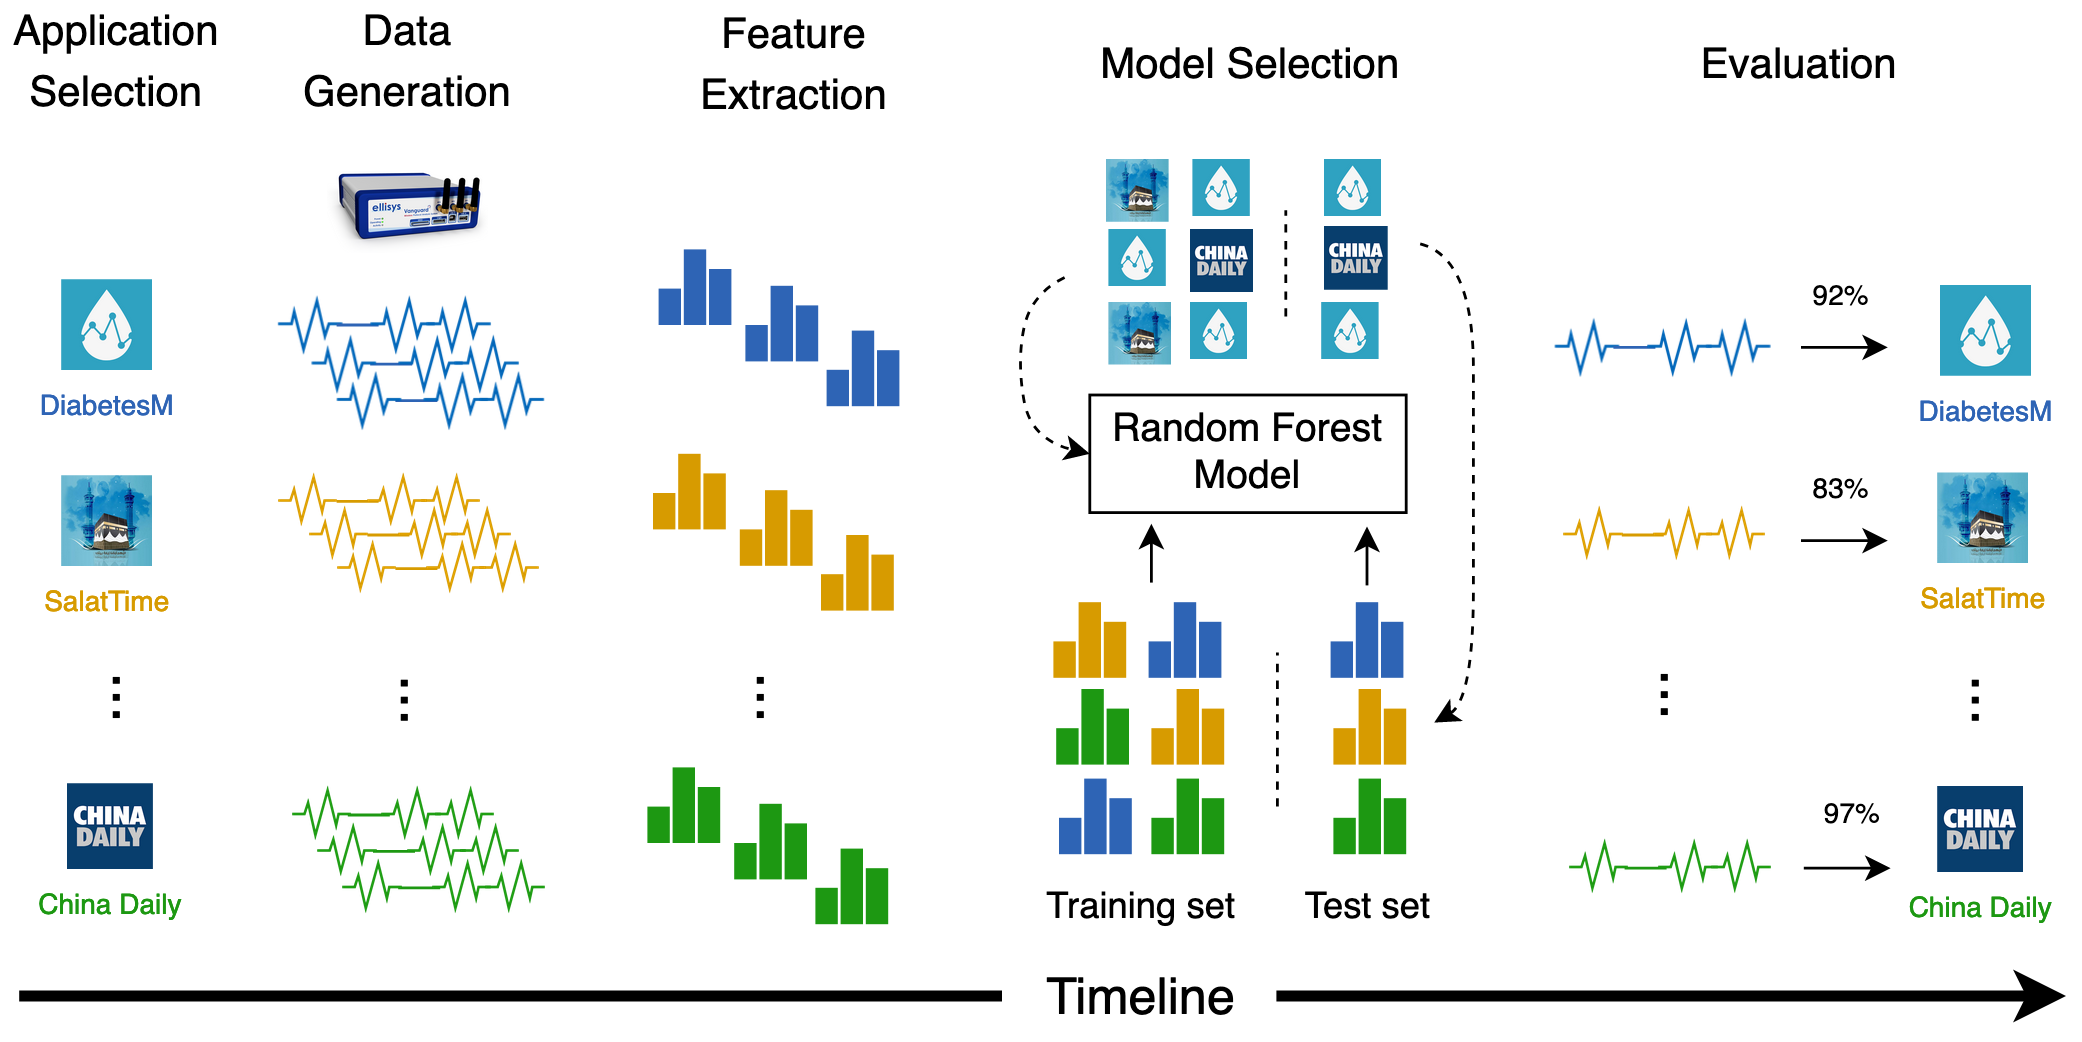
\includegraphics[width=0.98\textwidth]{figures/methodology.png}
 \caption{Attack broke down into 5 stages}
 \label{fig:attack_p1}
\end{figure}


 In the remaining sections, we describe each stage based on one particular smartwatch-phone pair: \textbf{Huawei-Pixel} from which specifications can be found in Tab.~\ref{tab:main_watch_spec}. Nevertheless the general approach applies for other smartwatch-phone pairs. 



\section{Application and Action Selection}
\label{sec:application_and_action_selection}
Applications are chosen based on three criteria:

\begin{itemize}
  \item \textit{Confidentiality}: Applications bearing specially sensitive information. Such as Health or Religious related applications, but also application that could show political interests or information about ethnicity.
  \item \textit{Popularity}: Popular applications based on the number of downloads and reviews, but also apps listed on famous websites that rank best smartwatches applications \cite{bestWearOSApp, bestWearOSApp2}.
  \item \textit{Nativity}: Applications installed by default on the smartwatch.
  \end{itemize}
  
Popularity and nativity ensure that the selected applications are representative of which application is more likely to be triggered, while confidentiality shows that the attack also works for specific sensitive targeted applications. Tab.~\ref{tab:app_examples} shows examples of selected applications, installed on the Huawei smartwatch, along with a short description and the selection criteria.
\\


\begin{table}[h]
\centering
 \begin{tabular}{@{}llll@{}} 
 \toprule
 Application & Description & Criteria  & Type\\ [0.5ex] 
 \midrule
 DiabetesM & Diabete Manager & Confidentiality & Health \\ 

 Maps & Google GPS navigation system & Popularity & Map \\

 Weather & Weather forecast  & Nativity & Other \\

 Spotify & Music Streaming & Popularity  & Other \\

 SalatTime & Islamic Prayer Manager & Confidentiality & Religious \\ 
 \bottomrule

\end{tabular}
\caption{Sample of selected applications installed on Huawei smartwatch with a short description, the criteria of selection and the application's type}
    \label{tab:app_examples}
\end{table}


We selected a total of 55 applications for our main stream experiment on the Huawei smartwatch. The complete list of these applications is given in the Appendix Tab.~\ref{tab:initial_Apps}. Fig.~\ref{fig:app proportio} shows the proportion of applications selected wrt. their criteria and types. We see that the most represented types of applications are Fitness apps and Health related apps, which is typically the kind of applications one would find on her smartwatch.

\begin{figure}[h]
\centering
\begin{subfigure}{.5\textwidth}
 \centering
  \includegraphics[width=0.65\linewidth]{figures/plots/Apps criteria repartition.png}
  \label{fig:sub1}
\end{subfigure}%
\begin{subfigure}{.5\textwidth}
  \centering
  \includegraphics[width=0.95\linewidth]{figures/plots/Apps typle repartition unfiltered.png}
  \label{fig:sub2}
\end{subfigure}
\caption{\textbf{Left:} Proportion of applications by criteria. \textbf{Right:} Proportion of applications by types}
\label{fig:app proportio}
\end{figure}


While the action of opening the application for the 55 initially installed application comes for free, we selected 17 extra actions on specific applications; we call them \textbf{in-app} actions. A complete list of these actions is given in the Appendix (see Tab. \ref{tab:selected_actions}).





\section{Data Generation}
\label{sec:data_generation}

We designed and implemented a system that allows an attacker to automatically generate a dataset from the applications selected in the previous stage. This automation system uses 5 devices:

\begin{itemize}
  \item \textit{Bluetooth Recorder}: Records Encrypted Bluetooth traces.
  \item \textit{Central Controller}: Orchestrates the simulation by synchronizing and controlling captures of Bluetooth traces and actions performed on the smartwatch.
  \item \textit{Bluetooth Recorder Controller (BR Controller)}: Controls the Bluetooth Recorder via a software.
  \item \textit{Smartwatch}: Performs application's action.
  \item \textit{Smartphone}: The Smartwatch's paired phone. 
\end{itemize}


\subsection{Automation Setup} We created a WLAN with no internet connection over Wi-Fi that connects the Central Controller to the smartwatch and the BR Controller. The BR Controller is connected via USB cable to the Bluetooth Recorder. The smartwatch is also connected to a smartphone via Bluetooth. Finally, we connect the smartphone to another WLAN via Wi-Fi with internet connectivity. This setup forces the smartwatch to use the phone as a default gateway over Bluetooth to access the internet while still being able to receive commands from the Central Controller via Wi-Fi. The setup is depicted in Fig. \ref{fig:automation_testbed}. 


\begin{figure}[H]
 \centering
 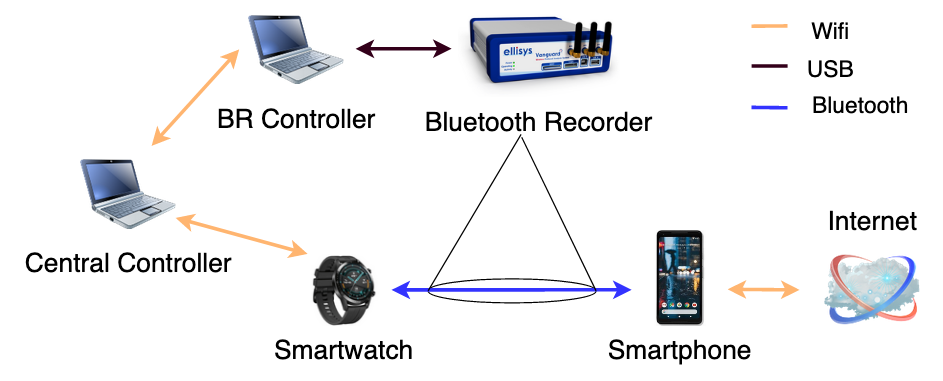
\includegraphics[width=0.7\textwidth]{figures/automation_testbed.png}
 \caption{Automation architecture.}
 \label{fig:automation_testbed}
\end{figure}

\\
\\

We specify that the smartwatch is charging at all time during data generation to ensure that it does not run out of battery, but also to allow persistent Wi-Fi connectivity, as we discussed in Sec.~\ref{sec:smartwatches}.
\\

While we change the smartwatch and smartphone for different experiments, we keep the same Bluetooth Recorder, BR Controller and Central Controller across experiments. We use Ellisys Vanguard BV1 for the Bluetooth Recorder, a Dell running Window 10 for the BR Controller having Ellisys Bluetooth Analyzer software installed and a ThinkPad running Ubuntu Bionic for the Central Controller.



\subsection{Automation Flow} For each action that is targeted by the attacker, the automation goes as follows. First, the Central Controller sends to the BR Controller the command to start recording the Bluetooth traffic of the targeted smartwatch-phone pair. Upon receiving the confirmation that the capture started by the BR Controller, the Central controller starts executing the action on the smartwatch. Once the action is done, the Central controller waits for a few seconds to ensure that the Bluetooth communication is finished. Then, the Central Controller sends a command to the BR Controller to stop and save the capture with the name of the application and the action which becomes the label of the capture. After having received the confirmation that the capture is saved, the Central controller sends a force-stop\footnote{\textbf{\textsc{force-stop}} ensures that the application is fully stopped and is ready for a fresh restart. We are convinced that this does not influence the real behavior of application loading since we can safely assume a garbage collector inside the smartwatch responsible of stopping left over processes after some period of time.} command such that the application is stopped and then waits a few seconds to ensure that the traffic reach a steady state. This procedure is repeated as many times as the attacker wants samples per action before switching to another action.


\subsection{Implementation}
On one side, we used \texttt{adb}\footnote{\textbf{\texttt{android debug bridge (adb)}} is a CLI tool that let a remote machine access an android device.} and \texttt{monkeyrunner}\footnote{\textbf{\texttt{monkeyrunner}} is a python API running on \texttt{Jython}. It provides simplified command to execute commands on an Android device.} on the Central Computer to control the smartwatch remotely. And on the other side, we used the python library \texttt{socket} to implement a server on the BR Controller which waits for commands sent by the Central Computer. The BR Controller uses \texttt{autoIt3}\footnote{\textbf{AutoIt Scripting Language} is a scripting language used to automate the interaction with the Windows GUI.} to execute the command on the Bluetooth Recorder software. The automation system runs checks (e.g. Bluetooth connection is up) to record any failure that might occur during the automation and keeps a log record.
\\

The whole system is composed of 1,350 Line of Code (LoC). 1,070 LoC run on the Central Controller: 620 python LoC and 550 yaml encoded commands to perform action on the smartwatch. On the other end, 280 LoC run on the BR Controller: 180 python LoC for the server and 100 AutoIt3 to automate commands on the software controlling the Bluetooth Recorder.

\subsection{Benefits}
The most important benefit from the automation system is the time consumption. We measured that to perform one capture, our automation system takes approximately one minute. If we assume an adversary that can generate capture as fast as the automation system, and has selected 24 actions with 25 samples per action, it would take him 10 hours in the data collection process. The time saving results in an easier dataset scalability and maintainability for an attacker. Moreover, the system is not prone to inattention error that human can have and thus might lead to a cleaner dataset. 
\\

We highlight that the system we designed is not only bounded to capture traffic between smartwatches and mobile phone. It can also be used to capture various kind of traffic. For instance, the system could be applied to audio fingerprinting, where the smartwatch would be replaced by the smartphone and the smartphone by earphones in Fig.~\ref{fig:automation_testbed}.

\subsection{Limitations and Alternatives}
The automation system only works on Android and WearOS. Unfortunately, \texttt{adb} and \texttt{monkeyrunner} are not available for other Operating Systems. Still, other alternatives exist. Tizen, running on Samsung devices, allows a remote connection with \texttt{sdb} (Smart Debug Bridge). However, the interaction with the smartwatch is much more constrained and allows only the command to open applications. 
\\


There are actions that the automation system is unable to control. For instance, if a push notification arises on the watch generating extra traffic, the system won't be able to detect it. The same goes for background updates. This results in noisier captures. There is still an option to filter out this extra noise by fetching the \texttt{btsnoop} log file on the smartwatch. However, we decided to not use this method as it might have significant discrepancies with the actual traffic sent, and also because not all smartwatches support \texttt{btsnoop}. We also note that keeping this background noise is a more realistic scenario of what we would find in the wild.
\\


Finally, automated actions might fail to capture real user pattern actions. However, this would also be true if a single user performs actions: the traces might be too specific to that user. 




\section{Feature Extraction}
\label{sec:Feature extraction}
In this section, we explain the third stage of the attack

\subsection{Basic Features Extraction} From our threat model, the attacker cannot see the payload's content of the traffic. However, nothing prevents him from passively recording, for each packet, the following characteristics: 
\begin{itemize}
    \item \textit{Direction}: The packet's direction. Either incoming (from phone to smartwatch) or outgoing (from smartwatch to phone).
    \item \textit{Length}: The packet length.
    \item \textit{Timing}: The time at which the packet is sensed by the attacker.
\end{itemize}{}


While the attacker can also see the Bluetooth packet type, we decided to not use this information because the Bluetooth protocol stack on smartwatches is in principle implemented on the Bluetooth chip and on the device's OS and thus is independent of applications.


\subsection{Statistical Features Extraction} 
From packets described by the tuple (\textit{Direction}, \textit{Length}, \textit{Timing}), we extracted statistics based on packet length and packet arrival time for each capture traces.
\\
 
 For packet length, we formed three groups: incoming packets only, outgoing packets only and non-null packets. On each group of packets, we computed the following six statistical quantities: The minimum, maximum, mean, standard deviation, number of packets in the group and the kurtosis\footnote{The kurtosis measures how heavily tailed is a distribution.}. In addition, we created features for each unique packet length, and by grouping the count of these unique packet length, we also computed the 6 statistical values above.
 \\
 
 For packets arrival time, we extracted the inter-arrival-time (IAT) between each packet having size more than 0, 46 and 1,005 length (see Sec.\ref{sec:model selection}). From these extracted IAT values, we also computed the same six statistical values.
 \\
 
 At this point, we are left with $6*3 + 1,005 + 6 = 1,029$ features on packet length and $3*6=18$ features on timing, thus a total of 1,047 features.
 \newpage



\section{Model Selection}
\label{sec:model selection}
In this section, we present the characteristics of the model.

\paragraph{Classifier.}
We use the \texttt{RandomForestClassifier} from the python library \texttt{sklearn}. Choosing Random Forest was motivated by the fact that this model is well known in traffic-fingerprinting to provide good performance~\cite{10.1145/3274694.3274697, k-fingerprinting, taylor2016appscanner}, but also, because it can deal well with high-dimensional data with sparse features and it gives an easy way to understand the importance of features. We set no restriction on the maximum depth of trees, Gini impurity for the splitting criteria, and the number of features to be considered in a split to the square root of the maximum number of features. We tuned these parameters by running a grid search algorithm and a cross-validation score. We also set the number of trees in the forest to 200.

\paragraph{Feature Filtering.} We setup the range of the unique packet length from 46 to 1,005. 1,005 is the maximum packet length in bytes that a Bluetooth packet can have. 46 was found by performing a grid search where we withdrawn each unique packet length feature from 1 to i until until i = 110. Since we got a stable accuracy until i=46 before dropping significantly, we expect that packets having length less than 46 are mostly controlled packets not related to applications. To further filter features, we leverage the RF architecture to extract the feature importance and filtered out all features with null importance. Consequently, we reduced the initial 1,047 features to less than a half. This allowed us to have a better insight of the features and speed up training and predictions from around 10\% to 40\%. 








\section{Evaluation}
\label{evaluation}

For each experiment, we follow the same guideline to evaluate the model: We first perform equalization across classes to ensure that all classes are perfectly balanced. We then performed 50 random split cross-validation with 75\% train and 25\% test to compute the accuracy and the 95\% confidence interval\footnote{computed as two times the standard deviation.} averaged over all predictions. Finally, we plot a confusion matrix of one realisation to gain more insight about the classifier.

\chapter{Attack Evaluation}
\label{chap:analysis_and_results}

In this chapter we provide an in-depth evaluation of the attack. Our main stream experiment is based on one smartwatch-phone pair: \textit{Huawei-Pixel}. Tab.~\ref{tab:main_watch_spec} shows the specifications of these two devices. In the first part of this chapter we analyze the results we get on this smartwatch-phone pair. After that, we see if the results also apply to two different pairs of devises (\textit{Fossil-Nexus} and \textit{AppleWatch-iPhone}). We finally summarize the results in the last Section.
\\

\begin{table}[ht]
    \caption{Specification of the main stream experiment's smartwatch-phone pair.}
    \label{tab:main_watch_spec}
\centering
\subcaption*{ \textbf{Huawei   -    Pixel}}
 \begin{tabular}{@{}lll@{}} 
 \toprule
  & smartwatch & phone \\ [0.5ex] 
 \midrule
 Manufacturer & Huawei & Google \\ 

 Model & Huawei watch 2 (LEO-BX9) & Pixel 2  \\

 OS version & wearOS 2.16 & Android v9  \\
 \bottomrule
\end{tabular}

\end{table}



\section{Application Opening Identification}
\label{sec:application opening identification}
We will first focus on simply targeting \texttt{open} action, i.e. fingerprint traces when we simply open one particular application. We believe that targeting this kind of action has two benefits: First, this is the simplest action and does not require any encoding in our automation system. But most importantly, opening is not influenced by a specific user pattern interaction with the smartwatch and would be the best candidate for successful fingerprinting in the wild.


\subsection{Filtering out Applications} 
\label{subsec:Filtering out Application}
Before starting our analysis, we suspect some applications to not send any data at opening. Which seems to be a realistic supposition as many applications should be self-sufficient at startup. To verify this, we ranked classes (i.e, opening action for different applications) according to the median of their total amount of data transfer against their accuracy. Fig.~\ref{fig:acc_ranked} shows the difference between ordering accuracy by class index (see Tab.~\ref{tab:initial_Apps}) and by data transfer size. From the right plot, we can clearly distinguish two clusters. The bottom left cluster contains applications that did not send data at opening, or at least not enough. Indeed, we can still see classes belonging to the bottom left cluster sending 212 bytes at the median. This could be due to background data communication such as push notification or background updates, or it could be that the amount of data sent by this application is not sufficient to classify it reliably. We notice that some applications have pretty high accuracy in this same cluster. This is explained by the fact that since they are only misclassified amongst themselves the random correct guess is more likely. Also, the classifier might have learnt a persistent background noise across different instances of the same class.
\\

\begin{figure}[H]
\centering
\begin{subfigure}{.5\textwidth}
  \centering
  \includegraphics[width=1\linewidth]{figures/plots/scatter_plot_accuracy_size_unordered.png}
\end{subfigure}%
\begin{subfigure}{.5\textwidth}
  \centering
  \includegraphics[width=1\linewidth]{figures/plots/scatter_plot_accuracy_size_ordered.png}
\end{subfigure}
\caption{\textbf{Left:} Classes accuracy ranked by class index. \textbf{Right:} Classes accuracy ranked by data transfer size median.}
\label{fig:acc_ranked}
\end{figure}


We filter out the of none-communicating application with the following formula:

$$ out = \{a:Pr(a_s<200) > 0.25\} $$

Where $a_s$  is the total amount of data (in bytes) captured when application $a$ is launched.
\\

Put into words, we filter out applications for which the amount of data captured when launched is less than 200 bytes more than 25\% of the time. We choose 200 because it seems to be the last value on the x-axis belonging to the first cluster (212 on Fig.~\ref{fig:acc_ranked}'s realisation). In fact, the fist class belonging to the second cluster has a median of 603, far beyond 200. 0.25 is chosen because we reckon that if the application really does not communicate, an intense background noise would not be present in more than 25\% of the captures.
\\ 

This particular filter removed 17 applications out of 55 in our dataset\footnote{The list of application indexes that does not communicate in out experiment are the following: \{1, 2, 4, 5, 12, 14, 21, 24, 25, 26, 32, 36, 37, 40, 45, 53, 55\} (see Tab.~\ref{tab:initial_Apps})}. We note that for two filtered applications (GooglePay and ASB mobile banking), we were unable to create user account\footnote{GooglePay because it required a password which might have influenced our experiment and ADB because it required an housing in New-Zeland, which unfortunately we do not have.}, which might affect the way the app normally communicate with the phone. Moreover, these applications are filtered only based on opening. This does not mean that another action does not trigger the communication enough to be fingerprinted, as we will see in Sec.~\ref{sec:in-App}. 
\\

By analogy to Fig. \ref{fig:app proportio}, we show the effect of filtering on the selected applications in Fig. \ref{fig:app proportion filtered}. We see that the type of applications affected the most by the filtering is the religious-related apps. Indeed, out of the four selected religious applications, two where simply offline excerpt of religious text. In contrast, the news, map and messaging application need to collect online resources and are not affected by the filtering.

\begin{figure}[h]
\centering
\begin{subfigure}{.5\textwidth}
 \centering
  \includegraphics[width=0.65\linewidth]{figures/plots/Apps criteria repartition filtered.png}
  \label{fig:sub1}
\end{subfigure}%
\begin{subfigure}{.5\textwidth}
  \centering
  \includegraphics[width=0.95\linewidth]{figures/plots/Apps typle repartition filtered.png}
  \label{fig:sub2}
\end{subfigure}
\caption{\textbf{Left:} Proportion of filtered applications by criteria. \textbf{Right:} Proportion of filtered applications by types}
\label{fig:app proportion filtered}
\end{figure}



\newpage

\subsection{Results on Apps Opening} After removing application that does not communicate at opening, we are left with 38 applications. We performed cross validation with 50 random splits on 38 samples per application, and got an averaged accuracy over all predictions of \textbf{96.8\% (+/- 2\%)}\footnote{We use this notation to denote the 95\% confidence interval.}. A realisation of a classification on this experiment is shown in Fig.\ref{fig:cm_open_huawei}. From the confusion matrix, we see that 31 apps have perfect accuracy score and the lowest accuracy score is 80\% (Fit, Qardio and Workout). 

\begin{figure}[H]
 \centering
 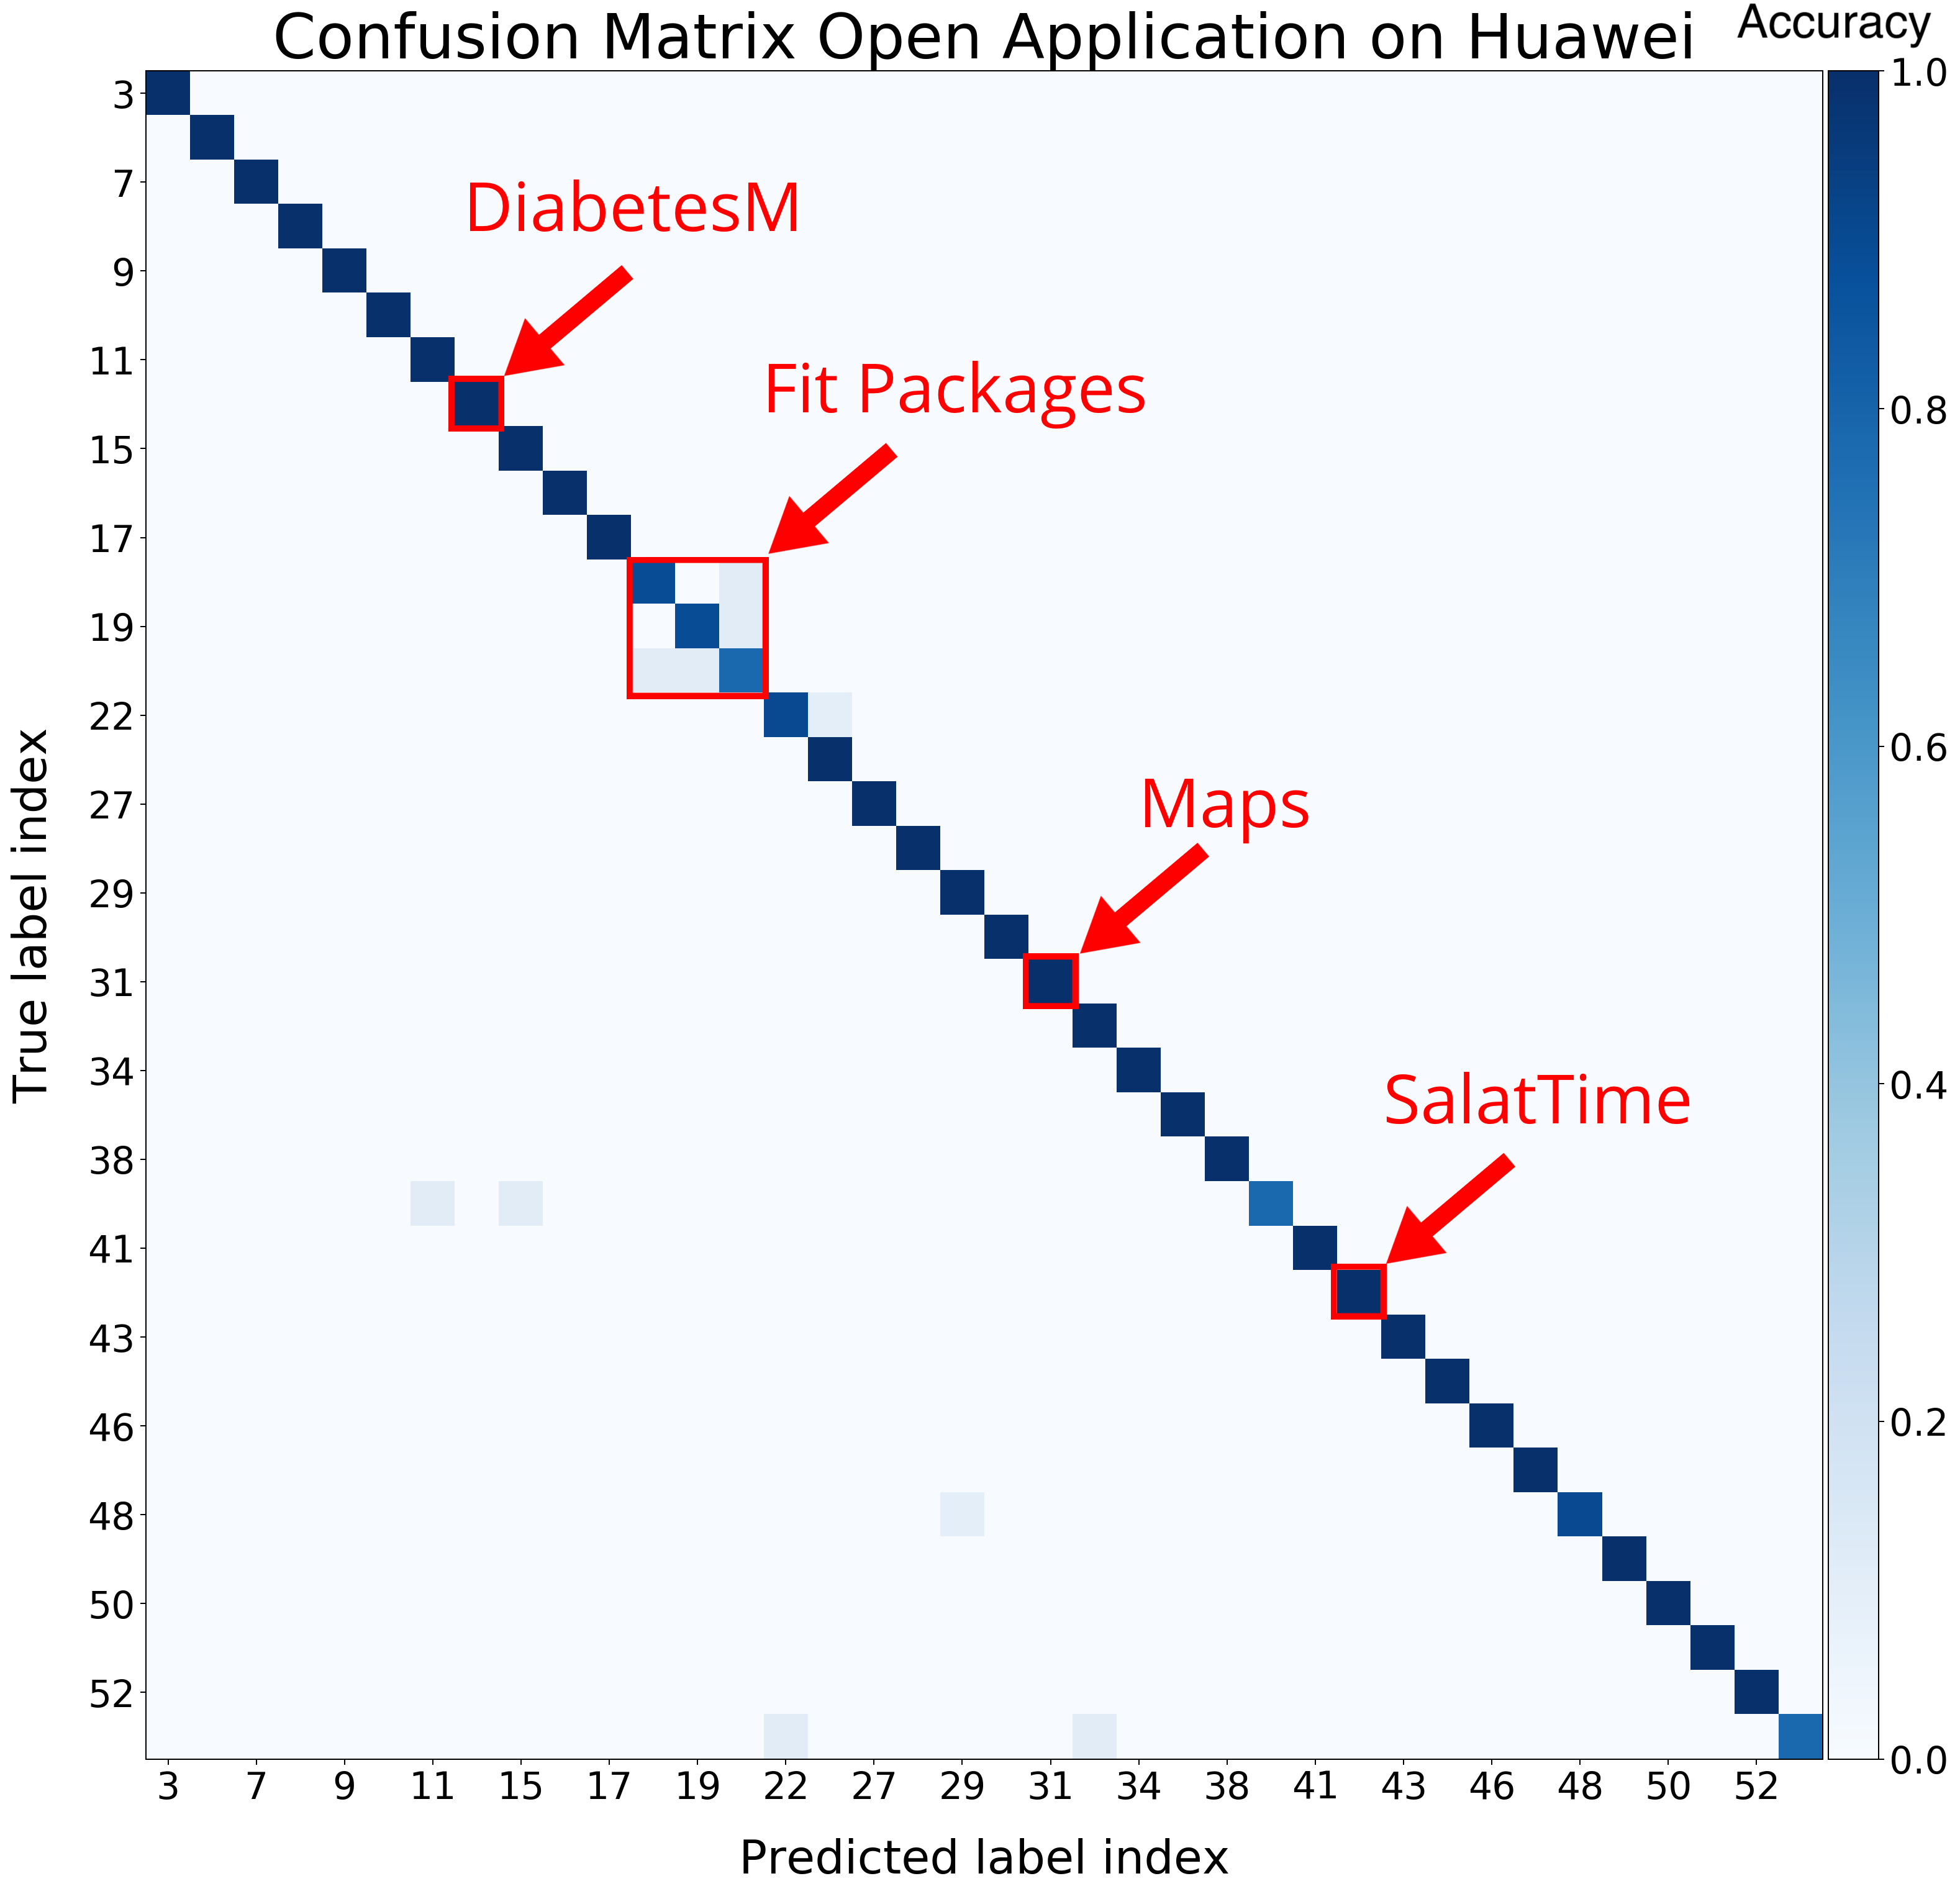
\includegraphics[width=0.70\textwidth]{figures/cm/Confusion_matrix_for_huawei_annoted.png}
 \caption{Confusion Matrix for open action on Huawei smartwatch.}
  \label{fig:cm_open_huawei}
\end{figure}


\newpage


\subsection{Number of Samples \label{data_set_size_per_class}
per Class vs Accuracy} Since generating data takes a long time, we investigate the impact of the number of samples per class on the accuracy to see how much accuracy an attacker might expect according to his dataset size. For this, we increasingly augmented the size of our dataset from n=2 to 30 samples per application. For each n, we picked 15 times n samples per class at random and performed 5 random split with 25\% test to extract the mean and the variance. We then average the mean and the variance over these 15 times. Fig.~\ref{fig:plot_accuray_dataset_size} plots the accuracy at different dataset size level.  We see that with a dataset size of 6 samples per class, we already achieve an accuracy of more than 90\% on average and with 11 samples per class more than 95\%. The variance also decreases. At 10 samples per class, we have less than 8\% accuracy lying inside the confidence interval, and at 24 samples per class, less than 4\%. 

\begin{figure}[ht]
 \centering
 \includegraphics[width=0.60\textwidth]{figures/plots/Accuracy_against_dataset_size_per_class_for_Huawei_final.png}
 \caption{accuracy against dataset size for 2 to 30 samples per application}
 \label{fig:plot_accuray_dataset_size}
\end{figure}






\section{In-App Action Identification}
\label{sec:in-App}
We saw in the previous Section that we can successfully identify applications at opening as long as it generates enough data. Now, we want to see at which point we can be precise in targeting specific actions within application. For instance, inside the application DiabetesM the user can perform several sensitive actions such as adding some glucose to his log book, or recording an insulin shot. Therefore, we launched the attack on a selected set of 17 specific in-app actions from six different applications (see  Tab.~\ref{tab:selected_actions}). We found out that over the 17 actions selected, the model has an accuracy of \textbf{68.2\% (+/- 7.1\%)}. Which is around 62\% more than the random guess. By looking at the confusion matrix in Fig.~\ref{fig:in-app huawei}, we see that actions within the same application are more subject to misclassification amongst themselves, which is still a good news for an attacker who plans to discover the installed application. Moreover, this does not apply for all applications. For instance, the application Lifesum has two actions (indices 70 and 71) and still achieve 100\% accuracy.


\begin{figure}[H]
 \centering
 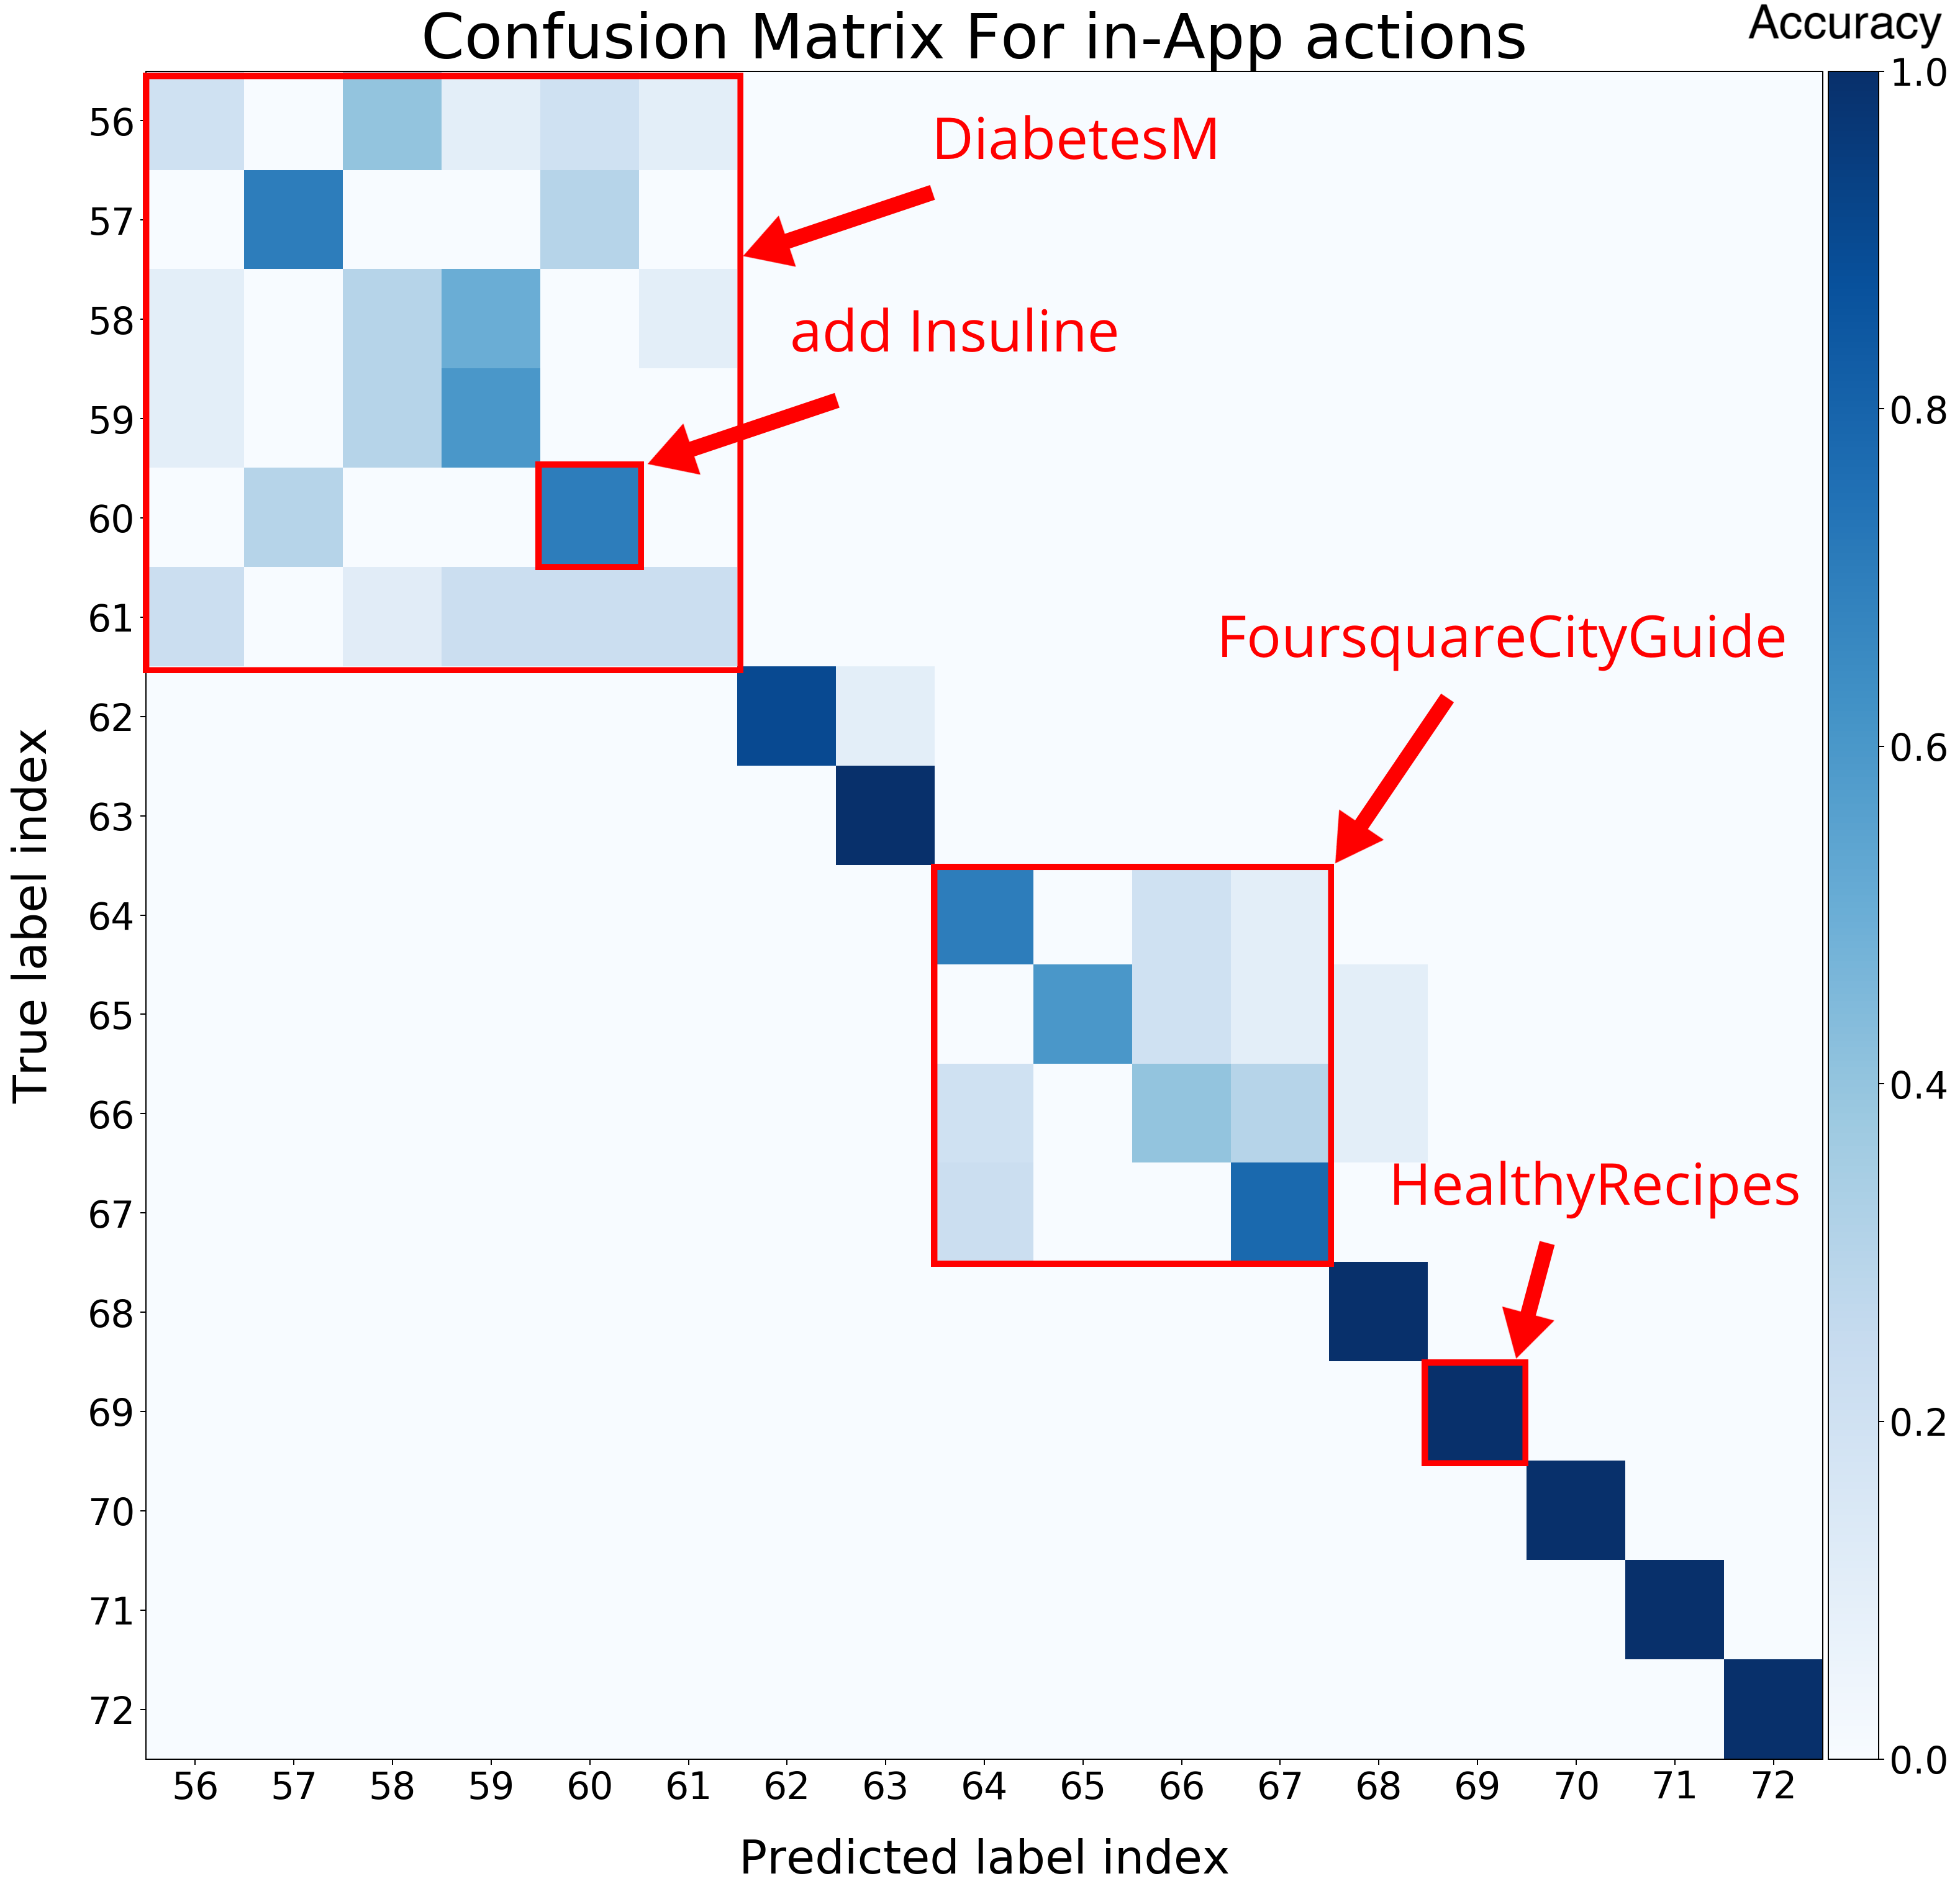
\includegraphics[width=0.7\textwidth]{figures/cm/all_inApp_action_annoted.png}
 \caption{Confusion matrix in-app actions on Huawei-Pixel.}
 \label{fig:in-app huawei}
\end{figure}


We note that the application HealthyRecipes was filtered out in Sec.~\ref{sec:application opening identification}. Even though at opening this app does not generate any traffic, we are still able to fingerprint it on a specific action (research Recipes in this case).









\section{Attack on Two Different Smartwatch-Phone Pairs}
We saw that the attack performs gracefully on one particular pair of devices. However, we want to show that the same attack also work on different smartwatch-phone pairs. Specifically, we selected two other smartwatch-phone pairs that differ in terms of Manufacturer, Model and OS version. Tab.~\ref{tab:extension_watch_spec} summarizes the specification of the two extra smartwatch-phone pairs. 
\\

\begin{table}[ht]
\begin{multicols}{2}
\centering
\subcaption*{\textbf{Fossil - Nexus}}
 \begin{tabular}{@{}lll@{}} 
 \toprule
  & watch & phone \\ [0.5ex] 
 \midrule
 Manufacturer & Fossil & LG Electronics \\ 

 Model & Q Explorist HR & Nexus 5  \\

 OS version & wearOS 2.16 & Android v6  \\
 \bottomrule
\end{tabular}
\subcaption*{\textbf{Apple Watch - iPhone}}
 \begin{tabular}{@{}lll@{}} 
 \toprule
  & watch & phone \\ [0.5ex] 
 \midrule
 Manufacturer & Apple & Apple \\ 

 Model & Apple Watch 5 & iPhone 8  \\

 OS version & watchOS 6.1.3 & iOS 13.3.1  \\
 \bottomrule
\end{tabular}

\end{multicols}
\caption{Specification of the smartwatch-phone pairs for the extended experiment.}
\label{tab:extension_watch_spec}
\end{table}


\paragraph{\textbf{Fossil - Nexus}.} For this experiment, we downloaded 35 applications out of the 38 applications tested on Huawei-Pixel (three of them were not compatible with the Fossil-Nexus pair\footnote{The three applications not compatible with the \textbf{Fossil - Nexus} pair are: \{3, 8,, 51\}, i.e. \{AppInTheAir, Camera, UARecord\}} at the time of the experiment). We collected 28 samples, performed 50 random splits with cross-validation and obtained an accuracy of \textbf{90.5\% (+/- 3\%)}. By looking at the confusion matrix in Fig.~\ref{fig:cm_fossil} we realize that the classes that are most misclassified are from the same native packages (Fit Package), this shows that these applications are very similar and reflects the possible difficulty to fingerprint actions belonging to the same application from Sec.~\ref{sec:in-App}. 


\begin{figure}[ht]
 \centering
 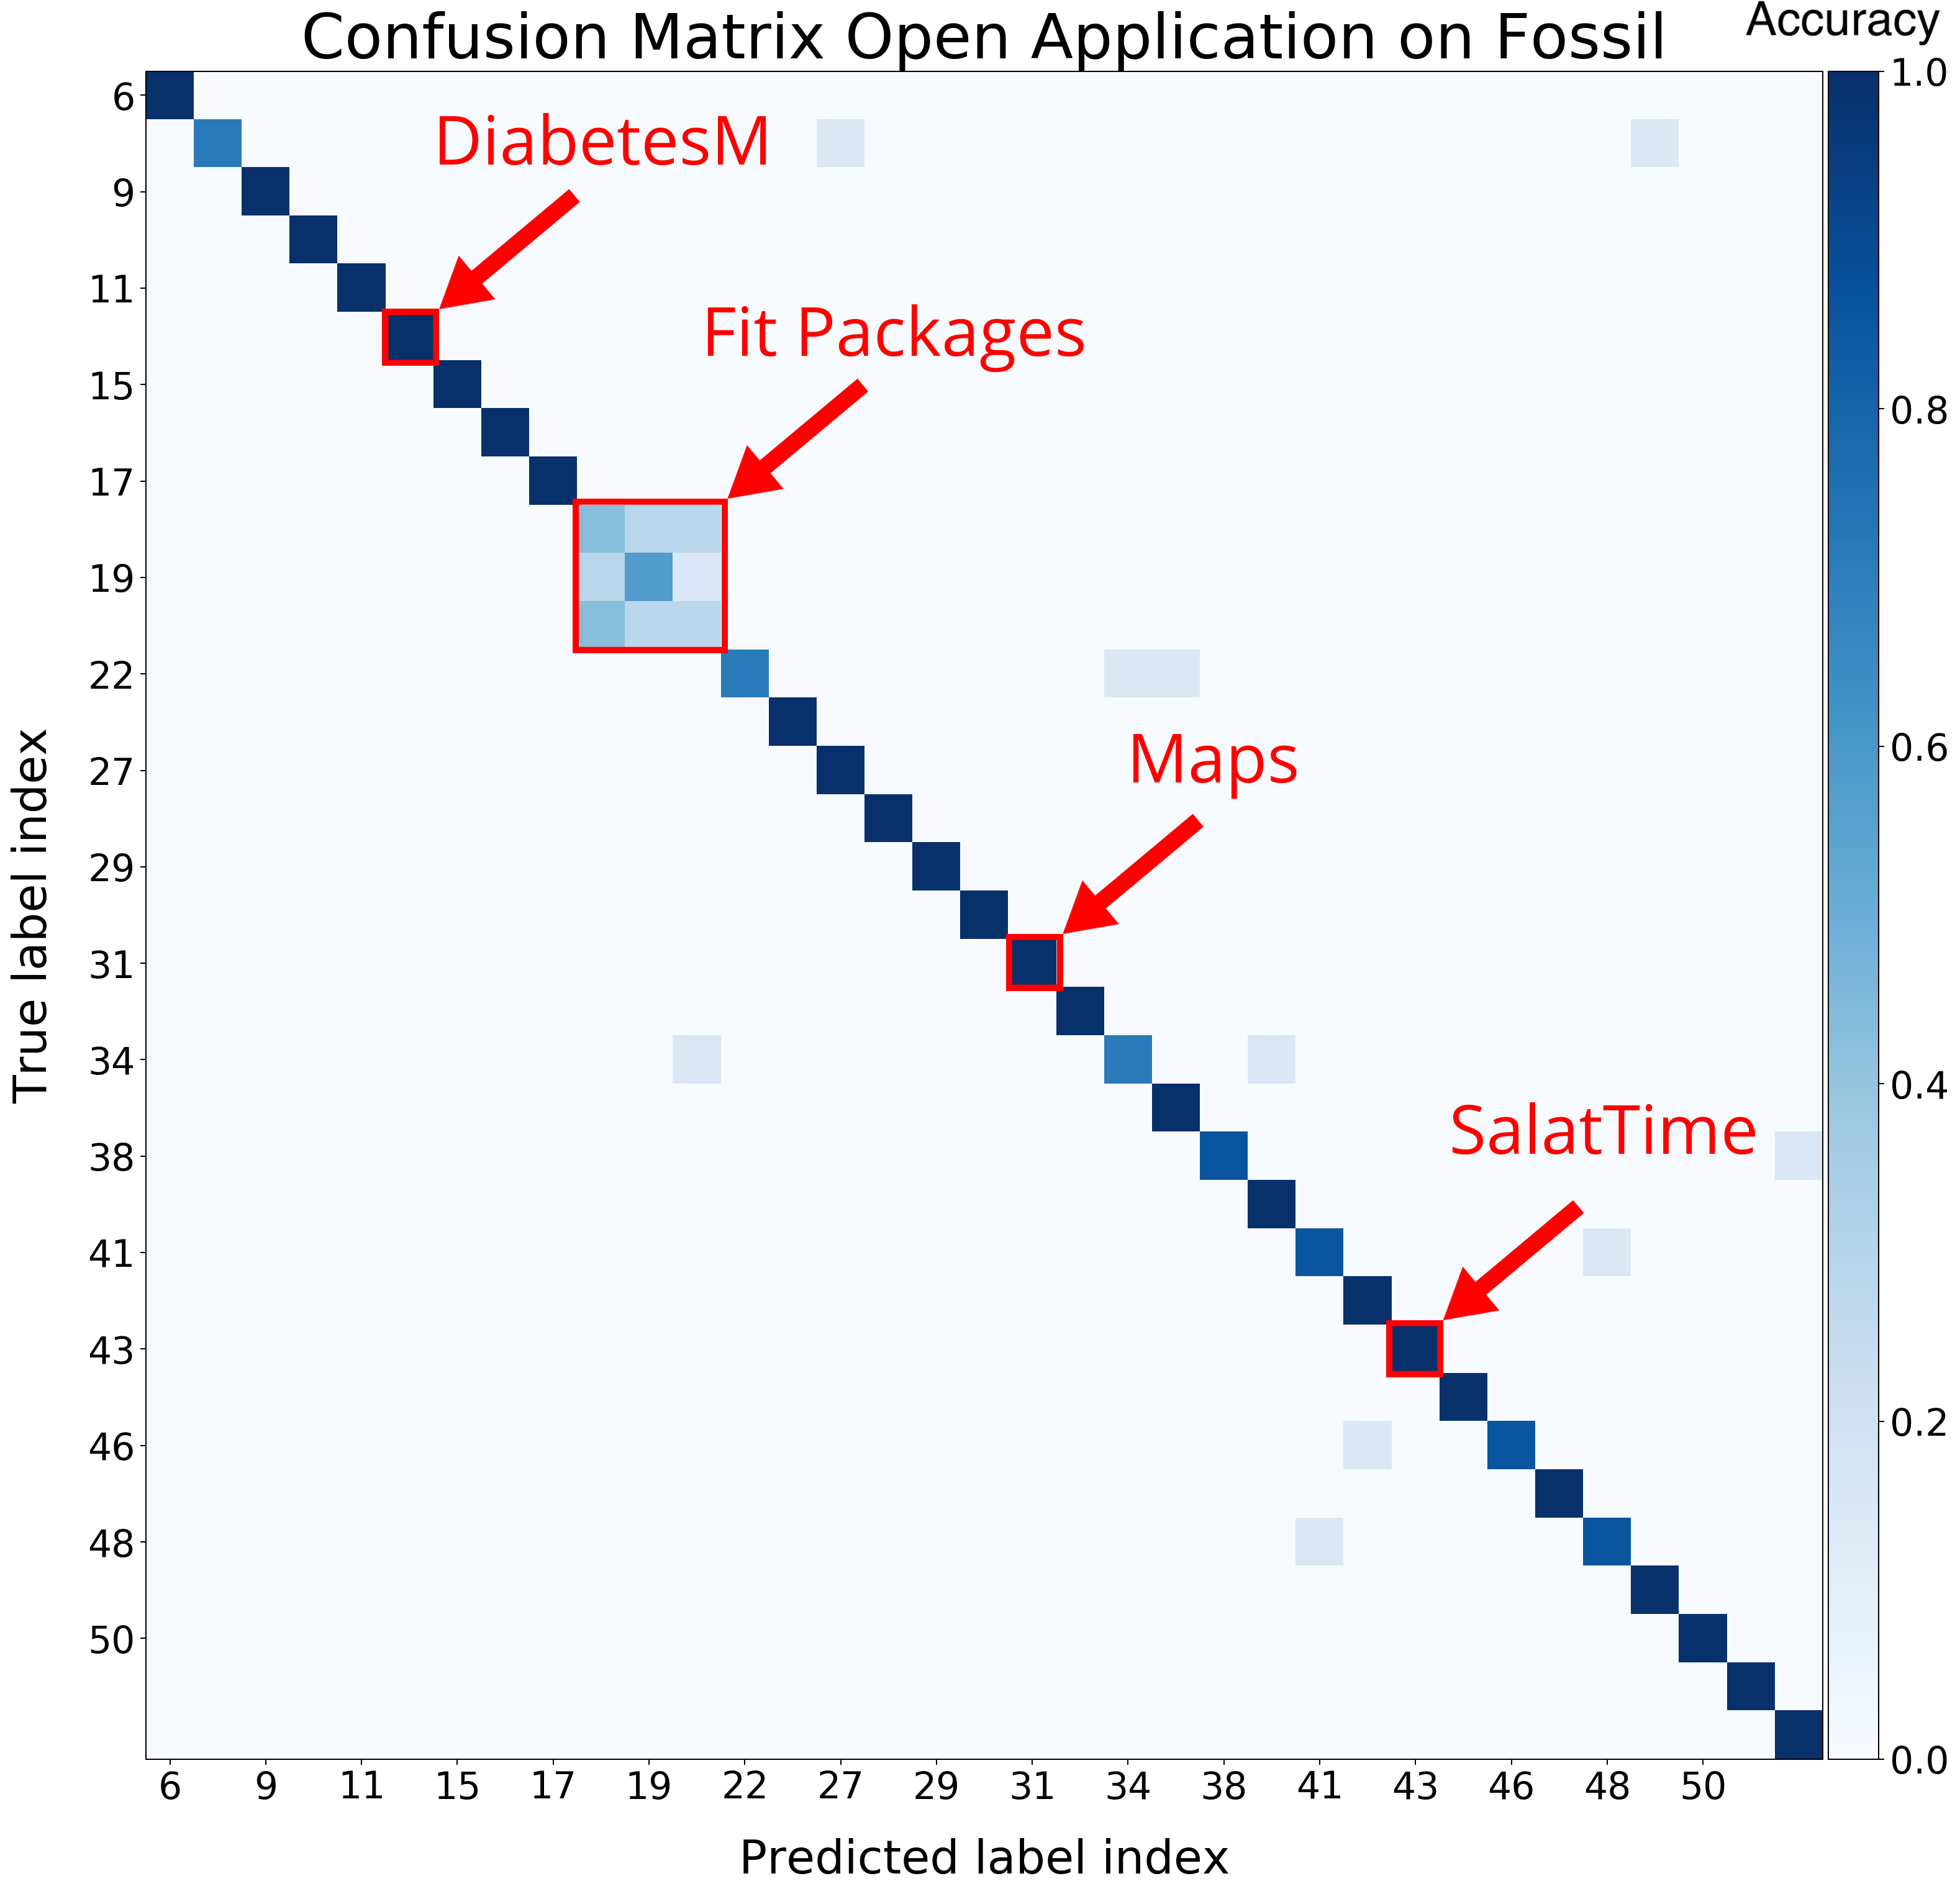
\includegraphics[width=0.70\textwidth]{figures/cm/Confusion_matrix_for_fossill_annoted.png}
 
 \caption{Confusion Matrix for open apps on Fossil smartwatch.}
 \label{fig:cm_fossil}
\end{figure}


\paragraph{\textbf{AppleWatch - iPhone.}}

We denote some differences between the AppleWatch - iPhone pair and the two previous pair of devices. First, the AppleWatch can transmit data over both Bluetooth Classic and Bluetooth LE requiring the attacker to possess a dual mode Bluetooth sniffer. Moreover, the connection is not persistent over Bluetooth Classic as it is on WearOS devices. This increases the difficulty to track the traffic. We also note that data transfer requiring low bandwidth tends to use BLE (apps such as PillReminder) in contrary, data transfer that requires higher bandwidth tends to use Bluetooth Classic (such as synchronizing electrocardiogram's data). In addition, as explained in Sec.~\ref{sec:data_generation}, we cannot automate the data generation and forces us to perform capture manually.  However, we show that even though these mechanisms seem to prevent an attack, we are still able to fingerprint the traffic with a good accuracy. Following the same guideline to evaluate the attack, we reach an accuracy of \textbf{88.7\% (+/- 7.5\%)} over 17 applications and 20 samples per application. The confusion matrix is shown in Fig.~\ref{fig:cm_iwatch}. We see that the lowest accuracy score is 40\% (20min.ch application). Out of the 17 applications tested, nine achieve perfect accuracy, such as ECG synchronization and RamadanTime.  




\begin{figure}[H]
 \centering
 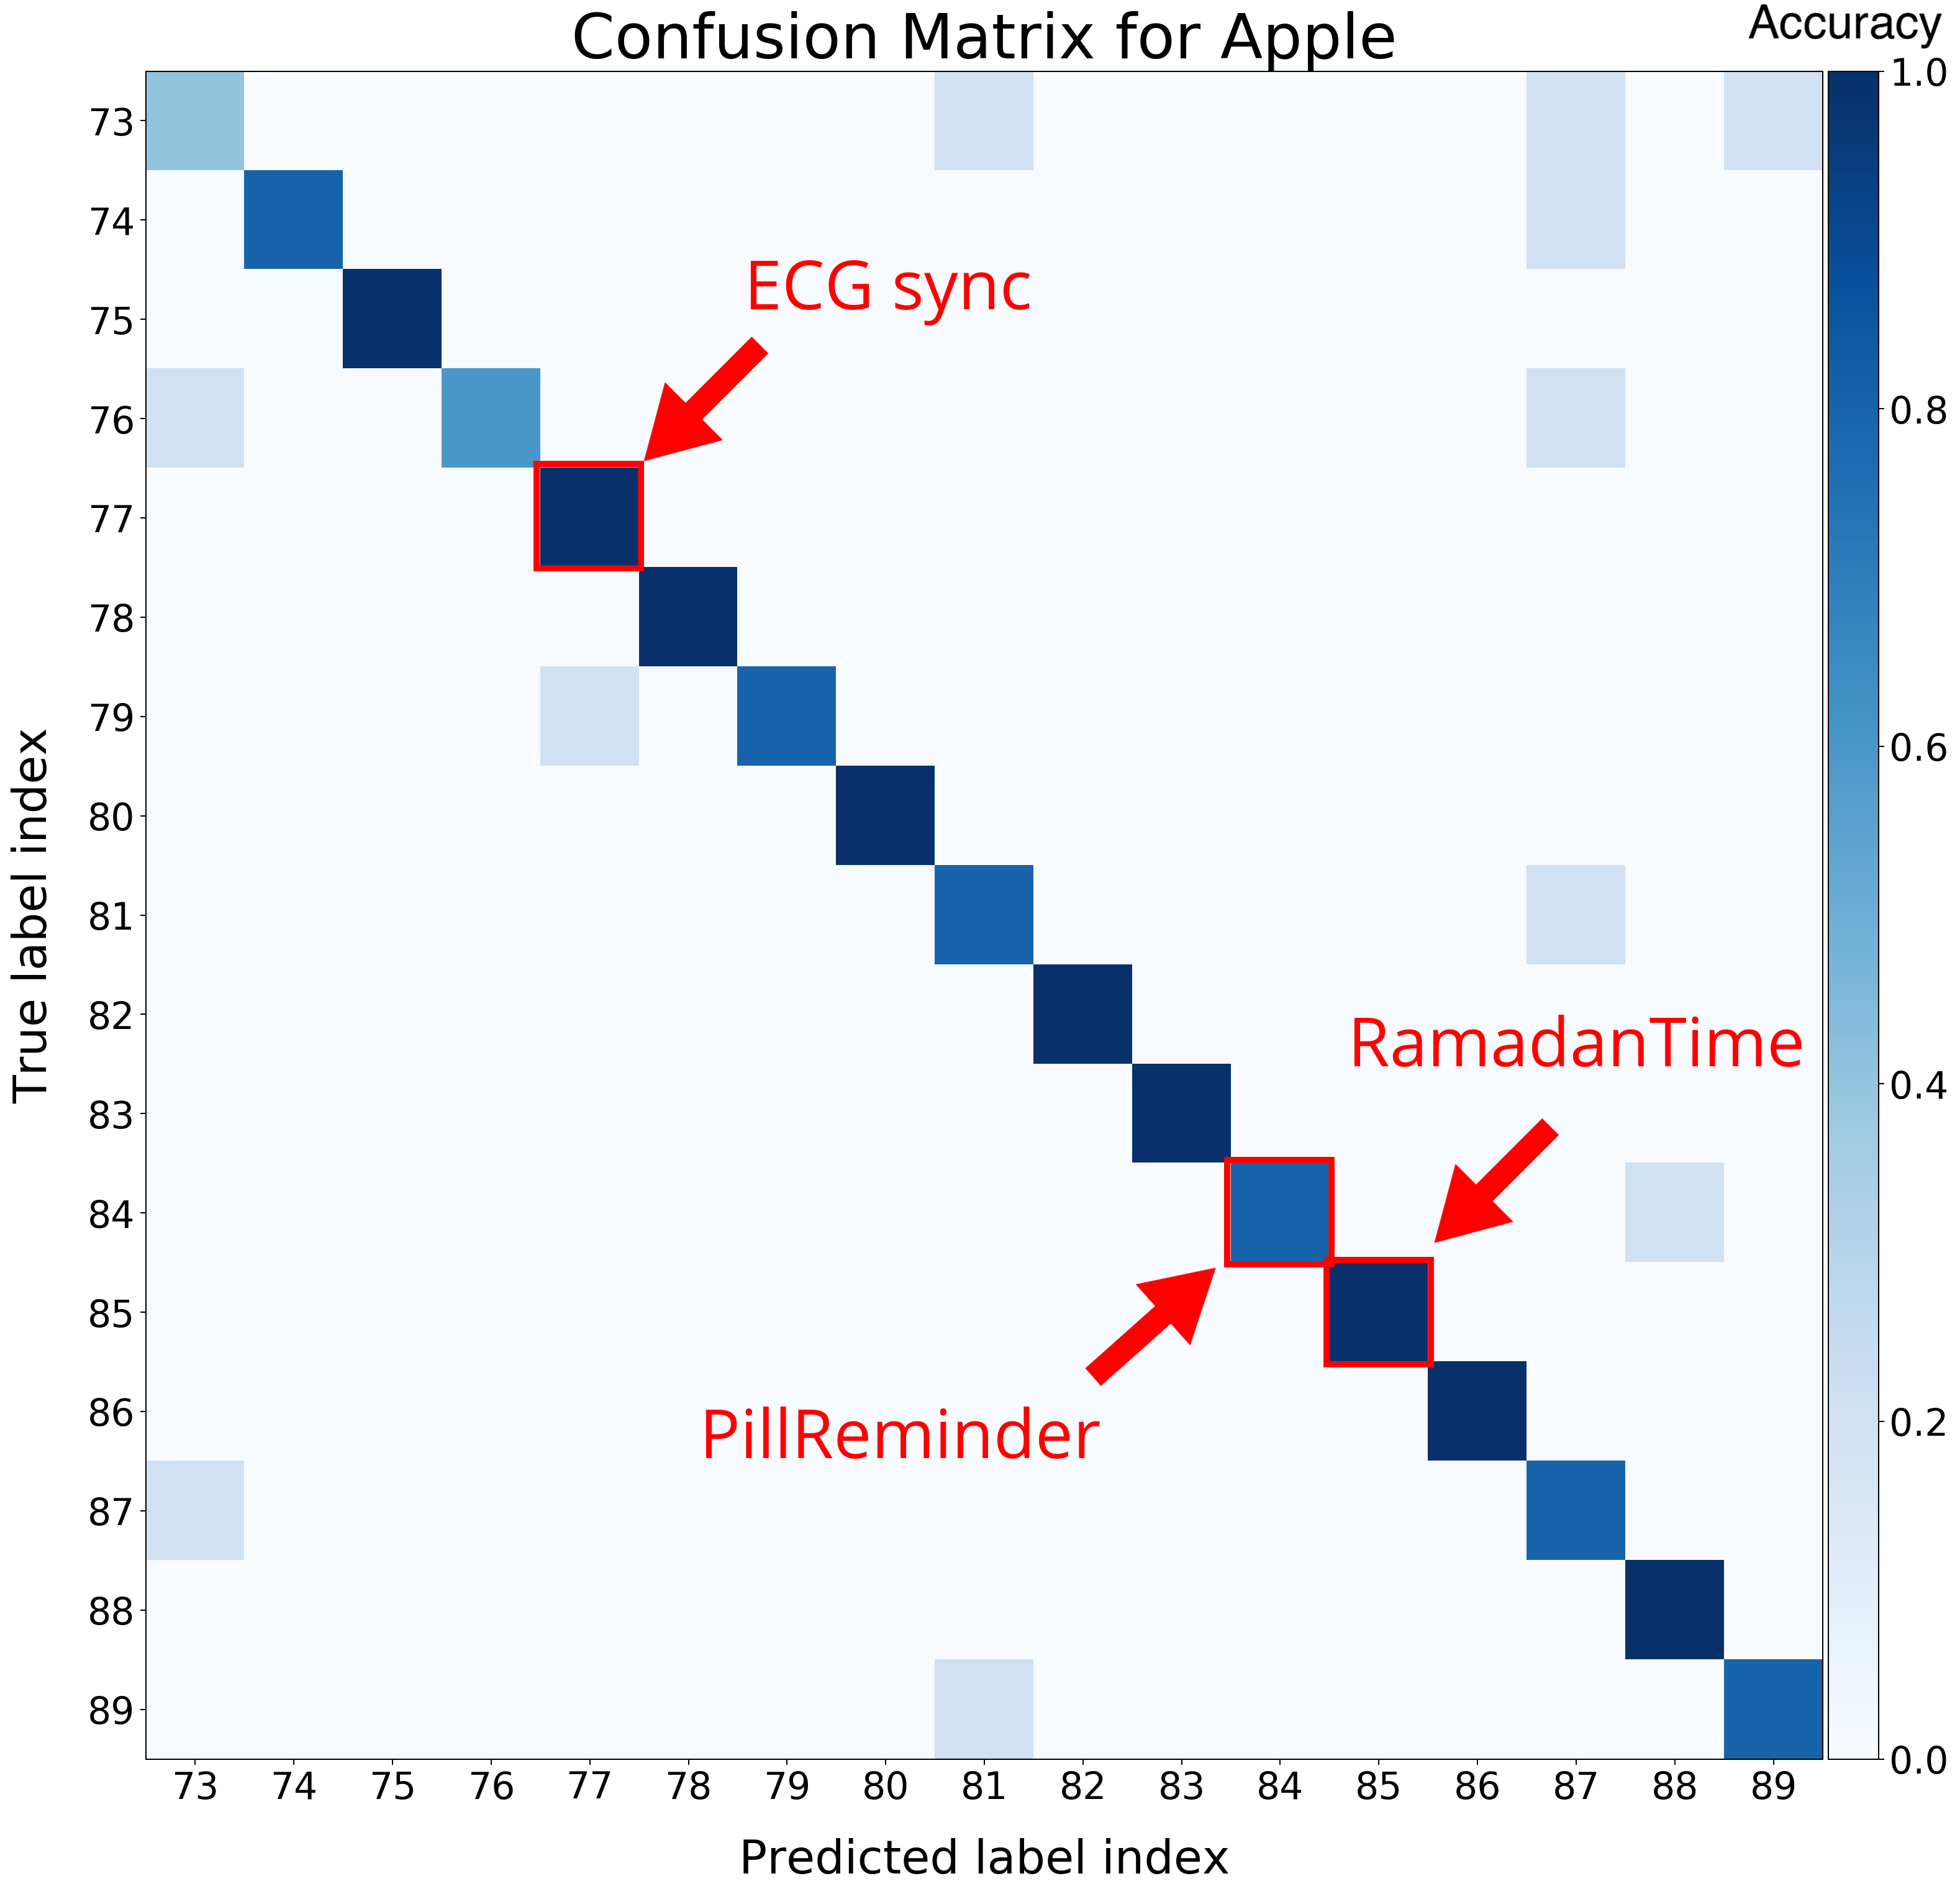
\includegraphics[width=0.7\textwidth]{figures/cm/Confusion_matrix_for_iwatch_annoted.png}
 \caption{Confusion matrix for Apple watch.}
 \label{fig:cm_iwatch}
\end{figure}






\section{Chapter Summary}
\label{chapter summary}
In this Chapter, we saw that encrypted Bluetooth traffic of smartwatches is highly subject to fingerprinting. Actions related to the same application might be hard to differentiate but are not likely to be confused with actions related to other applications. We also saw that the attack works on different devices. We give a summary of the results in Tab.~\ref{tab:results summury}. 
\\

\begin{table}[ht]
\centering

 \begin{tabular}{@{}llcccc@{}} 
 \toprule
  smartwatch-phone & actions targeted & accuracy & 95\% conf. & nb. class & nb. samples/class \\ [0.5ex] 
 \midrule
 Huawei-Pixel & opening  & 96.8\% &  2\% & 38 & 38\\ 

 Huawei-Pixel & in-app & 68.2\% & 7.1\% & 17 & 39\\
 
 Huawei-Pixel & opening \& in-app & 88.5\% & 2.6\% & 55 & 38\\

 Fossil-Nexus & opening & 90.5\% & 3\% & 35 & 28\\
 
 AppleWatch-iPhone & mix & 88.7\% &  7.5\% & 17 & 20  \\
 
 \bottomrule
 
\end{tabular}
%\caption{Sample of selected applications with short description and the criteria of selection}
 %   \label{tab:app_examples}

\caption{Results on the different experiments run in this Chapter.}
    \label{tab:results summury}
\end{table}


However, one question remains: How performs the attack on the whole set of actions on Huawei-Pixel? We explored opening and in-app actions but not both at the same time. Thus, we run the attack one more time on the set of all actions. This time, since the dataset is bigger, to ensure a good evaluation of the model, we used 200 random splits for cross-validation. The overall accuracy score is \textbf{88.5\% (+/- 2.6\%)}. The lowest F1 score of a targeted action is \textbf{30.78 (+/- 25.02)} whereas the best F1 score achieves \textbf{100\%}. We give samples of score achieved by different classes in Tab.~\ref{tab:rank summarize}.  We give an overall ranking and their associated score over the 55 actions in the Appendix (see Tab. \ref{tab:attack ranking}).
\\

\begin{table}[H]
\centering
 \begin{tabular}{llllll} 
 \toprule
 application name & action & F1 score & precision & recall \\ [0.5ex] 
 \midrule
FoursquareCityGuide & coffee & \textbf{30.78 (+/- 25.02)} & 32.96 (+/- 28.62) & 30.57 (+/- 28.12)\\
DiabetesM & addInsulin & 74.19 (+/- 18.89) & 73.85 (+/- 23.32) & 76.38 (+/- 26.60)\\
Shazam & open & 95.08 (+/- 9.28) & 99.17 (+/- 5.67) & 91.69 (+/- 16.07)\\
 Lifesum & addFood & 99.51 (+/- 3.78) & 99.13 (+/- 6.87) & 99.95 (+/- 1.41)\\
DiabetesM & open & \textbf{100.00 (+/- 0.00)} & 100.00 (+/- 0.00) & 100.00 (+/- 0.00)\\
 \bottomrule
\end{tabular}
\caption{Samples extracted from the overall ranking in Tab.~\ref{tab:attack ranking}. }
    \label{tab:rank summarize}
\end{table}
\chapter{Generalization of the Attack}
\label{chap:Generalization}

So far, our attack is only based on one single environment. The attacker trains and tests his attack on the same pair of devices with data collected at roughly the same point in time. In this chapter, we explore a generic context, where an attacker test his attack on other devices and with time delays.

\section{Transferability}
We want to show that an attacker learning on a particular smartwatch-phone pair can also detect applications on another smartwatch-phone. This would benefit greatly an attacker, since one single pair of devices would allow him to target many possible others. 
\\

We took the Huawei-Pixel and Fossil-Nexus dataset, from Chapter~\ref{chap:analysis_and_results}, learned the model on one pair, test on the other and vice versa. To allow a fair comparison, we selected a subset of 35 overlapping applications and performed equalization such that the two pairs have the same amount of samples per class. We used all the dataset of one pair for training and tested on all the dataset of the other pair. We achieve \textbf{80.3\% (+/- 0.7\%)} accuracy when training on Huawei and testing on the Fossil and \textbf{85.5\% (+/- 1.3\%)} vice versa. We note that training on Fossil leads to lower accuracy. This is explainable because the overall accuracy when only Fossil is tested is lower. Thus the Fossil dataset is noisier and more difficult to predict. We show the Confusion Matrix in Fig.~\ref{fig:cm transferability}. 
\\

\begin{figure}[h]
\centering
\begin{subfigure}{.5\textwidth}
  \centering
  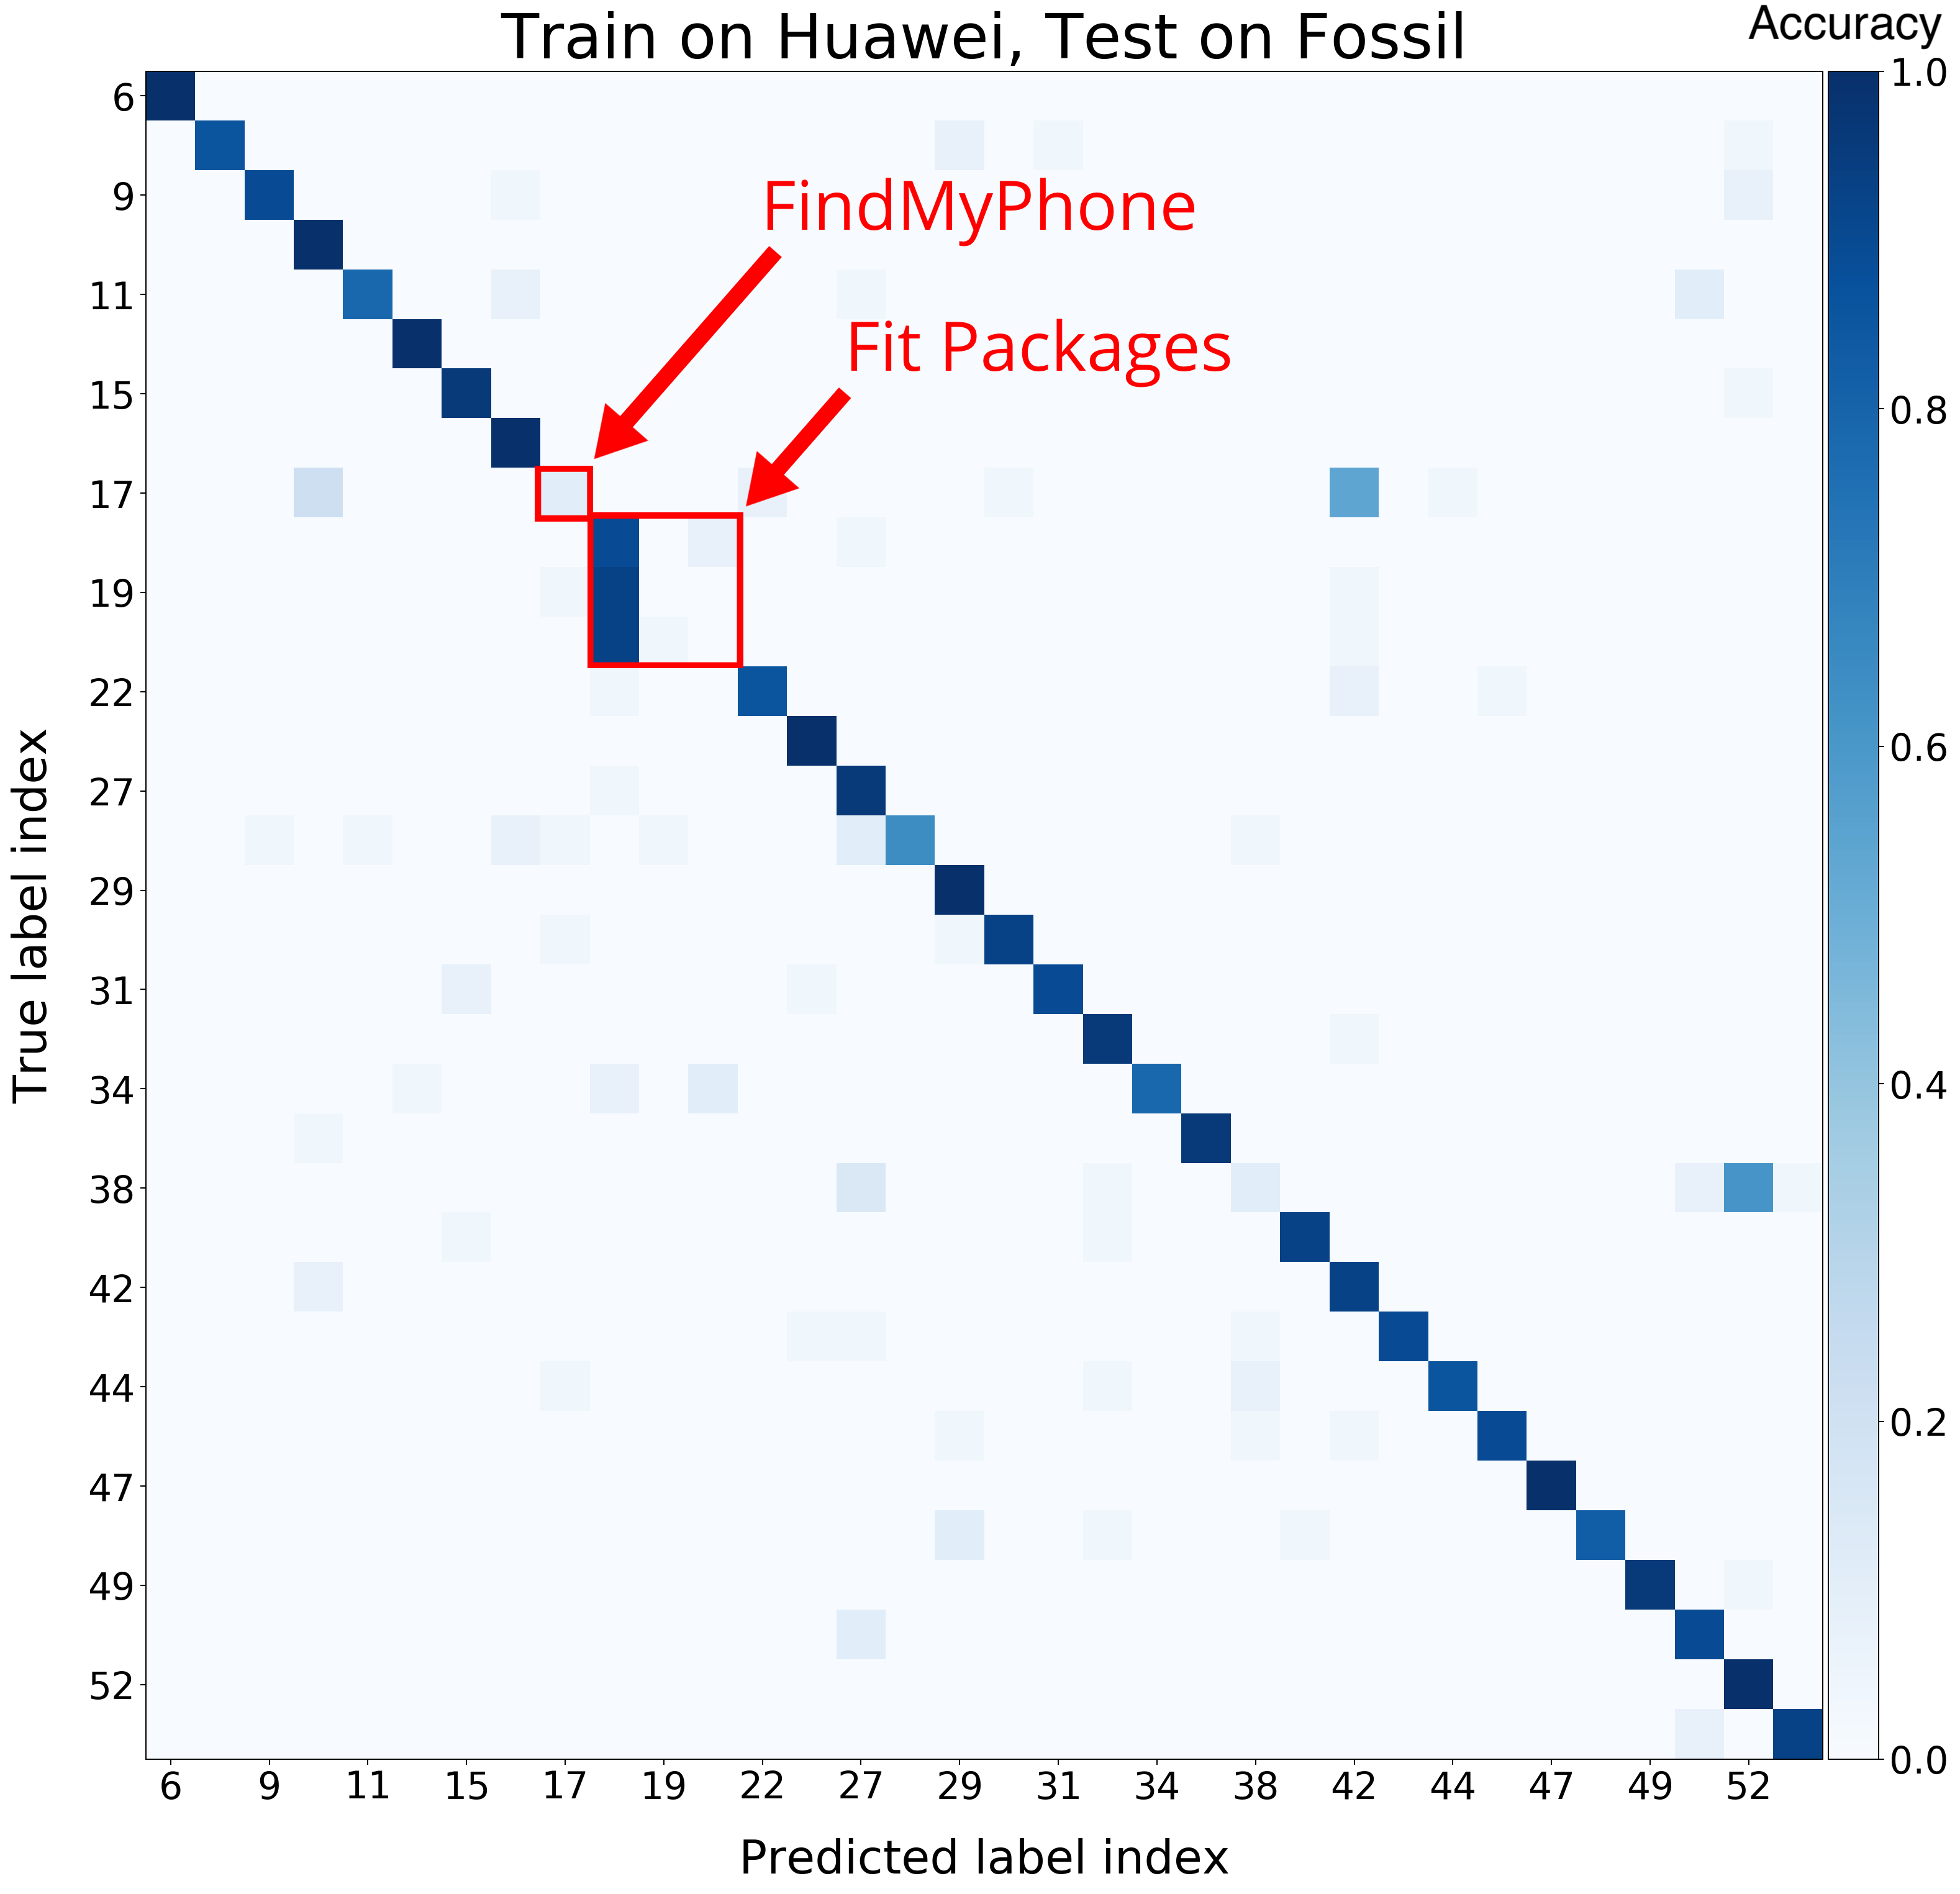
\includegraphics[width=1\textwidth]{figures/cm/Confusion_matrix_train_with_Huawei_test_with_Fossil_annoted.png}
\end{subfigure}%
\begin{subfigure}{.5\textwidth}
  \centering
  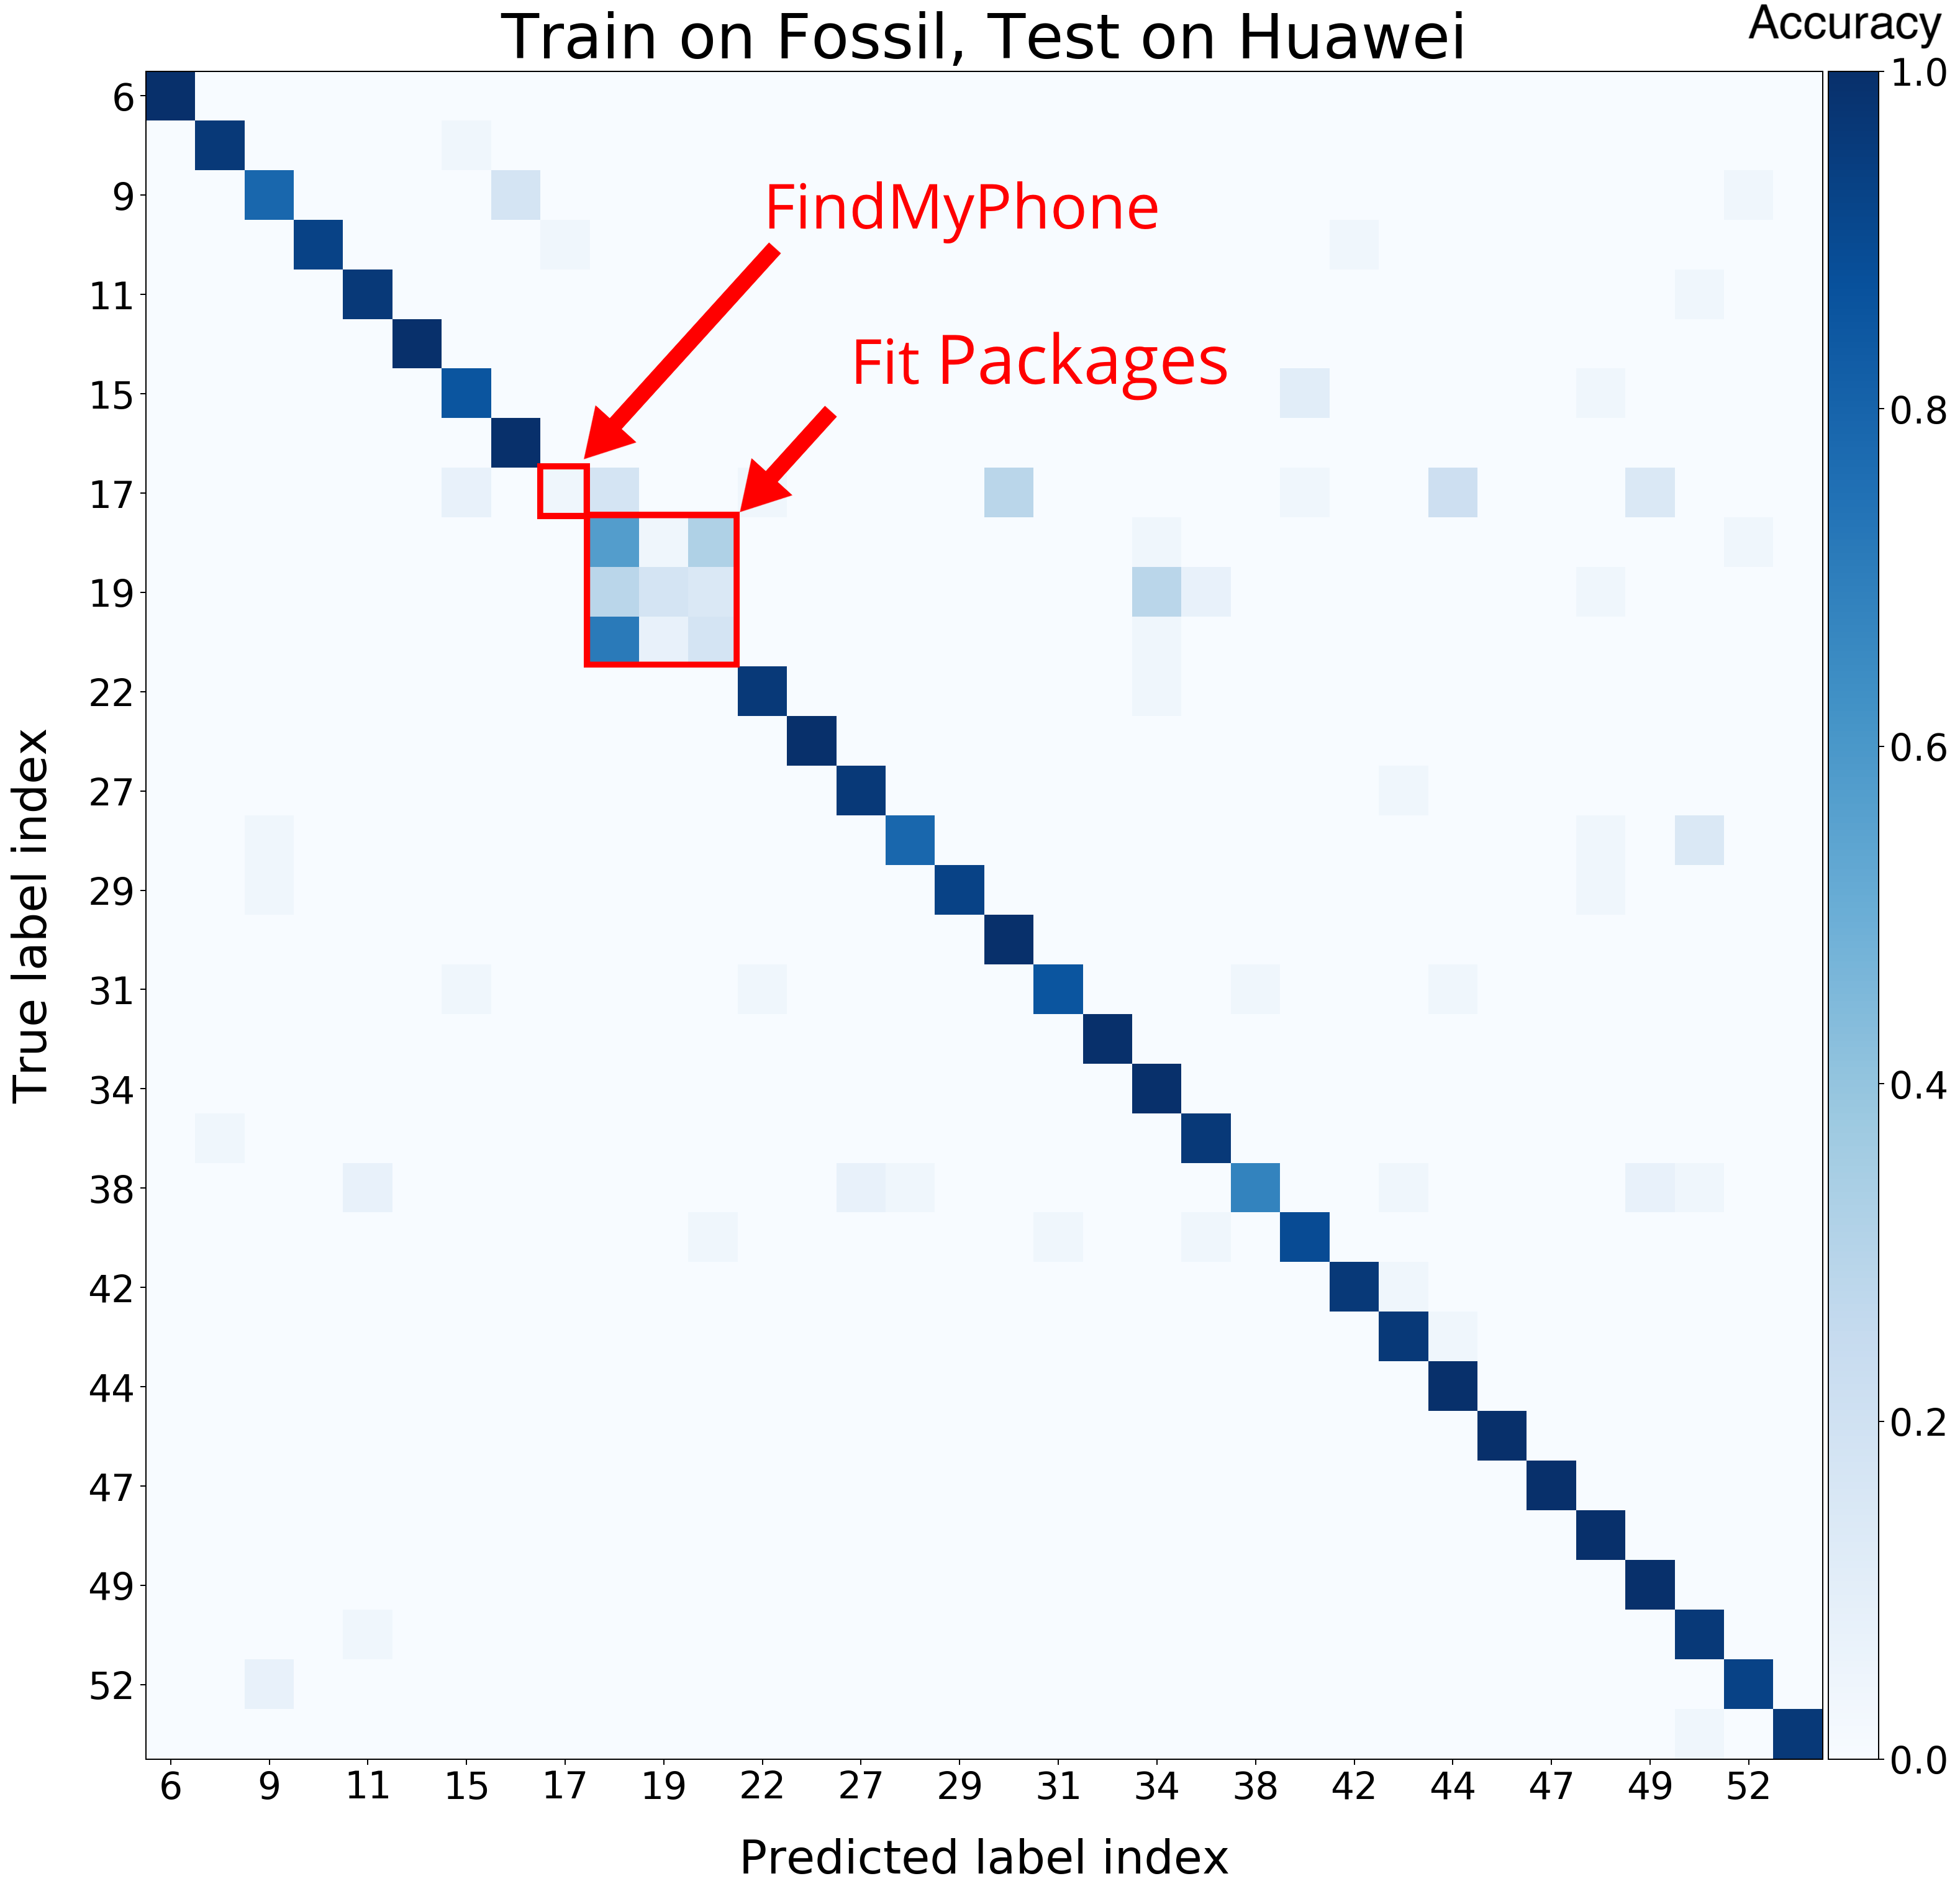
\includegraphics[width=1\textwidth]{figures/cm/Confusion_matrix_train_with_Fossil_test_with_Huawei_annoted.png}
\end{subfigure}
\caption{\textbf{Left:} Attacker learn on Huawei, test on Fossil \textbf{Right:} Attacker learn on Fossil, test on Huawei}
\label{fig:cm transferability}
\end{figure}
\newpage
We notice that only few applications lower the accuracy. FindMyPhone, for instance does not achieve more than 15\% accuracy score in both experiments. FindMyPhone\footnote{\textbf{FindMyPhone} is an application on smartwatches that rings the phone when triggered.} is an application that relies highly on the phone and its operating system, thus explaining why we do not expect to achieve more accuracy on this application. Moreover, we also see that apps coming from the Fit packages also do not achieve good results. We knew already that these apps are noisier since they are from the same package. By grouping the Fit packages into one entity, we found an accuracy of \textbf{86.1\% (+/- 0.7\%)} and \textbf{90.1\% (+/- 1.1\%)} for Huawei train and Fossil test and vice versa. Overall, the attack transfers very well apart from few specific applications.

\section{Evaluation over Time}
\label{sec:eval over time}
One could argue that the model we develop is too specific to one particular environment. i.e. the training set of the attacker is acquired in the same condition than the testing set. Network conditions might vary, the content of applications might change over time (such as maps or news applications), and application updates might also impact the traffic\footnote{Unfortunately, we did not track software updates of application and OS updates. However, updates happen more often than we expected. We recorded that in six days (from April 22nd 2020 to April 28th 2020), 11 software updates from different packages have been updated in the background.}. In 2014, Juarez et al. formulated the same critic towards WF, using previous work, they show that after 5 days accuracy dropped from around 80\% to less than 50\%\cite{juarez2014critical}. Taylor et, al. also formulated critics along these lines for MAF~\cite{taylor2017robust}. Therefore, even though an attacker can update his dataset to keep fresh data, we ask ourselves how accuracy will decrease with ageing and how frequent should an attacker updates its dataset.
\\

We collected, over 33 days, 11 set of captures at 4 days interval except for the first two days where we also performed captures. We initially took a subset of 33 applications and generated 10 captures per application on a "capture" day. However, at day 20, we realised that an update arose on the applications belonging to the Fit package, making them not transferring data anymore. So we put these apps aside and continued with only fingerprintable applications. The blue line in Fig.~\ref{fig:accuracy over time} shows the accuracy over time when trained with the dataset at day 0 and test with the dataset at day n. The red dotes are the accuracy when the training and testing dataset are from the same day. 

\begin{figure}[H]
 \centering
 \includegraphics[width=0.7\textwidth]{figures/plots/Accuracy_over_time_c08to1_train_only0_bis2.png}
 \caption{Accuracy over time }
 \label{fig:accuracy over time}
\end{figure}

\newpage

First, we note that the accuracy when we train and test on the same day have a slight variations (+/- 3\%) across days this confirmed our experiment on dataset size (see Sec.~\ref{data_set_size_per_class}). As expected there is a small accuracy decrease of 3.7\% on average between the blue line and the red dotes showing that, over time, the attack is weakened. Now, the question is how is this noise distributed over the classes. To see that, we averaged the accuracy loss over all days separated by class (See Fig.~\ref{fig:acc gain overtime}). We distinguish two things from this plot. First, except few apps that have small positive accuracy gain (or no gain), most apps are loosing accuracy over time. Moreover, one package has almost 50\% accuracy loss: DCLMRadio, a christian radio broadcast application. We explain this by observing the following: this application directly fetches a large amount of data from a remote sever at startup, and we suspect that errors occur frequently on their server which changes radically the communication scheme for specific days. In addition, two other apps show significant losses of more than 10\%: Google Map and Outlook.
\\
\begin{figure}[ht]
 \centering
 \includegraphics[width=0.70\textwidth]{figures/plots/accuracy_gain_per_class_when_mix_trained_j=all.png}
 \caption{Accuracy gain per class averaged over all days.}
  \label{fig:acc gain overtime}
\end{figure}

To reduce the accuracy drop caused by ageing, we trained the model on the first three days of the experiment instead of the first day alone, but with keeping the same dataset size to ensure fair comparison. We reproduce the graph from Fig.~\ref{fig:accuracy over time} and \ref{fig:acc gain overtime} in Fig.~\ref{fig:learning extension over time}.


\begin{figure}[h]
\centering
\begin{subfigure}{.5\textwidth}
  \centering
  \includegraphics[width=1\textwidth]{figures/plots/Accuracy_over_time_c08to1_train_only0_bis2_mix.png}
\end{subfigure}%
\begin{subfigure}{.5\textwidth}
  \centering
  \includegraphics[width=1.05\textwidth]{figures/plots/accuracy_gain_per_class_when_mix_trained_j=all_mix2.png}
\end{subfigure}
\caption{\textbf{Left:} Accuracy over time when trained with day 0, 1, and 2 \textbf{Right:}Accuracy gain averaged over time by class}
\label{fig:learning extension over time}
\end{figure}

\newpage

By doing this learning adjustment, we lower the average accuracy drop between current and delayed training from 3.7\% to 0.37\%. We can see now that the blue curve follows the red dotes. Interestingly, we could even achieve better results at day 20, which shows that the model can also learn better features when the training environment is changed. Indeed, if we look at the right part of Fig.~\ref{fig:learning extension over time}, we see that four applications achieved better results on average. Amongst them, ChinaDaily, a news app where content is updated frequently. Also, we could significantly lower the loss of DCLMRadio application (leftmost bar) by about a half. 
\\

To answer the question how frequent an attacker should refresh its dataset, we can say that after 32 days, 3.7\% is not a huge loss. However, some applications might suffer much more from ageing than others, and therefore an attacker wanting to be consistent over all its targeted actions might want to perform more frequent updates. Moreover, to counterbalance the effect of ageing, and to perform less updates, an attacker might want to train his model over few days.


\chapter{Long-run Attacks}
\label{chap:towards_a_realistic_attack}

Until now, we considered the attacker dealing with single-action captures. In practice, an attacker might record possibly many different actions within one single, longer capture (because he cannot a priori know when each action starts and stops): we name this \textit{long-run} captures. This scenario extents to cases where a targeted victim stays for a while close-by to the attacker such as in an office. In this chapter, we test our attack on long-run captures. In addition, we discuss and address different challenges emerging from this setting: How to distinguish noise from actual actions, how to cut the traffic such that we do not miss the beginning or the end of an action. 

This section is structured as follows: First, we describe the experiment on long-run captures. Then, we explain the attack methodology. Finally, we present the results.

\section{Experiment Description}
In this chapter, all the experiments are done with the Huawei-Watch pair on 50 different actions: 33 openings and 17 in-app actions (see Sec.~\ref{sec:application opening identification} and Sec.~\ref{sec:in-App}) . We use the same setup as in Sec.~\ref{sec:data_generation} and extended our automation system by 200 LoC on the Central Controller to support long-run capture (see Sec.~\ref{sec:data_generation}). In our implementation, the automation system has three simulation modes: 

\begin{enumerate}
    \item \textbf{Deterministic inter-action launching}: The time in-between two consecutive actions launched on the smartwatch is deterministic 
    \item \textbf{Uniform inter-action launching}: The time in-between two consecutive actions launched on the smartwatch is randomly uniformly distributed
    \item \textbf{Interaction pattern inter-action launching}: The time in-between two consecutive actions launched on the smartwatch follows a specific user interaction pattern.
\end{enumerate}

We used the two first modes exclusively for training and validation, and the last mode exclusively for testing. In the two first modes, we arbitrarily set the waiting time mean of two consecutive actions to 50 seconds. For the third mode, we adjust the waiting time to follow the daily user interaction pattern based on the work of Liu, et al \cite{10.1145/3081333.3081351}. Fig.~\ref{fig:user_interaction_pattern} compares the daily user pattern interaction from the original paper and our simulation. Due to technical reasons, instead of considering portion of one hour, we considered slots of 20 minutes, and performed three times the experiment to have a total of 24 hours capture; which corresponds to 2.2 GB.





\begin{figure}[H]
\centering
\begin{subfigure}{.5\textwidth}
  \centering
  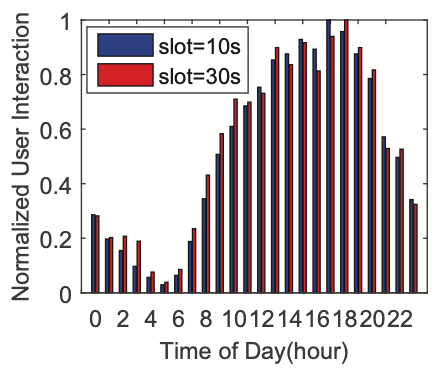
\includegraphics[width=0.92\textwidth]{figures/user interaction.png}
\end{subfigure}%
\begin{subfigure}{.5\textwidth}
  \centering
  \includegraphics[width=1.05\textwidth]{figures/plots/reproduced_user_interaction_level.png}
\end{subfigure}
\caption{\textbf{Left:} Daily user interaction pattern (from Liu, et. al). \textbf{Right:} Reproduced user interaction level on performed action triggered}
\label{fig:user_interaction_pattern}
\end{figure}
\\
 

Moreover, Liu et. al, reported that some applications are more likely to be triggered. Therefore, we give higher prior launching probability for actions belonging to the popular apps described by Liu et. al in Fig.~\ref{fig:popular apps}. However, due to the lack of information about how more frequent these applications are, we arbitrarily set their prior probability to be 1.5x higher than other apps. The rest of the applications are launched with equiprobability.


\begin{figure}[H]
 \centering
 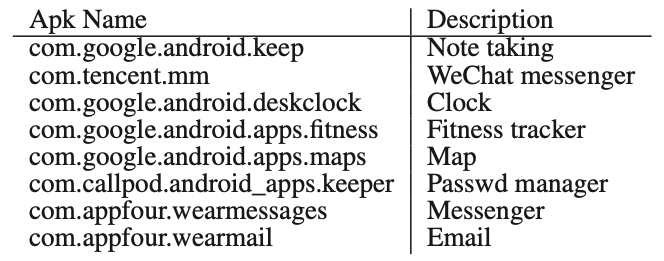
\includegraphics[width=0.5\textwidth]{figures/popular apps.png}
 \caption{Popular applications on smartwatches more likely to be triggered by a user (from Liu, et.  al~\cite{10.1145/3081333.3081351}).}
 \label{fig:popular apps}
\end{figure}


\section{Methodology}
\label{sec:longrun methodology}
Three building blocks composed the attack. First, the long-run capture is processed by a Sequence Splitter, whose job is to output chunks containing traffic of one single action performed on the smartwatch. A classifier then takes these chunks as input and outputs the probability of each chunk to belong to a specific class. Finally, the Decision Maker gives the final output from the vector probability. In all the modules, mechanisms are deployed to prevent noise to be wrongly classified as actions. Fig. \ref{fig:longrun methodology} gives an overview of the attack on a long-run capture.


\begin{figure}[H]
 \centering
 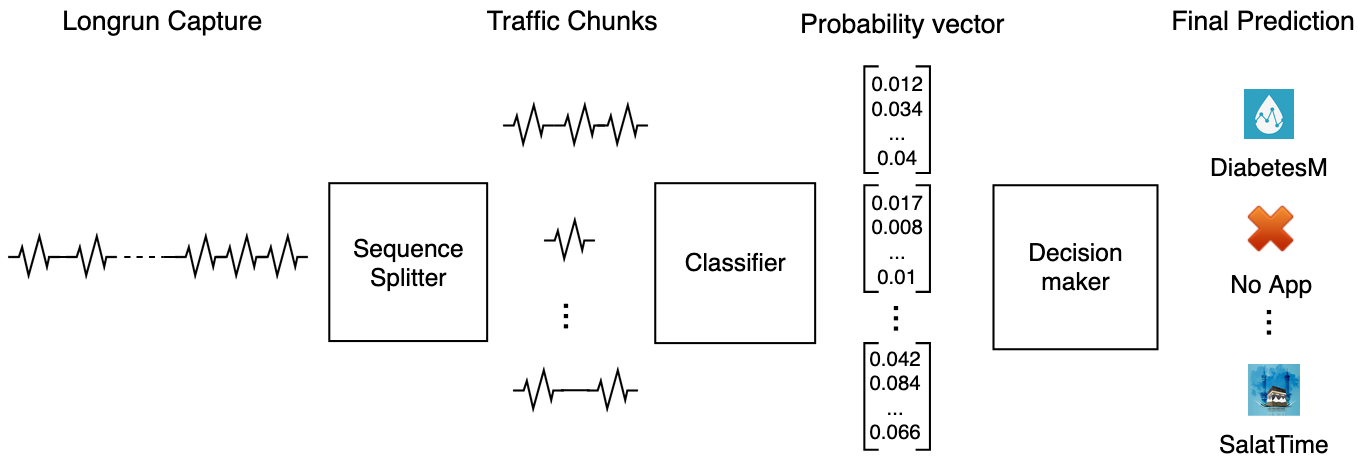
\includegraphics[width=0.98\textwidth]{figures/longrun overview 2.png}
 \caption{Overview of the attack on long-run captures.}
 \label{fig:longrun methodology}
\end{figure}

\paragraph{Sequence Splitter.} To process the long-run capture, the Sequence Splitter first identifies the points where an action might start (i.e. starting points). These starting points are found by moving a Sliding Window with length T seconds on the long-run capture. A point is considered as a starting point if the sum of packets length within the Window is more than N bytes. We choose N=200 bytes since action's traffic must contain more than 200 bytes (to pass the filter we designed for single-action capture, see Sec.~\ref{subsec:Filtering out Application}). We choose T=15 seconds based on training on the two first simulation modes and by intuition on the duration length of the traffic generated by a performed action\footnote{It is interesting to note that both parameters have different impacts on precision and recall for the two different action types (i.e. openings and in-app action)}. Then, from each starting point we determine the termination point, where the potential action might stop. A termination point is found if for a period of more than T seconds we do not receive any packets of length more than N bytes. Here, we choose N=46 because we consider packets with length smaller than 46 as noise (see Sec.~\ref{sec:model selection}), and T=10 in the same way as for the starting points. We note that the Sequence Splitter is designed such that an attacker does not need to wait the end of the long-run capture to make a prediction, and can process the long-run capture in real-time.


\paragraph{Classifier.} We build the same classifier as the one for the attack on single-action capture (see Sec.~\ref{sec:model selection}), yet with the following changes: we added one more class on top of the 50 targeted classes. This class serves as a filter to flag noise not related to targeted action. During our experiment, we realised that sometimes applications also generate traffic at closing, which is less fingerprintable so we decided to include these types of traffic to the extra class. Also, to attenuate the effect of ageing, we reused the dataset which spanned over 33 days (see Sec.~\ref{sec:eval over time}). Finally, the classifier does not output directly the prediction, but a probability vector representing its confidence about a particular class.

\paragraph{Decision Maker.} The Decision Maker takes has input the probability vector and outputs the majority voting only if the highest value in the vector is above a specific threshold. Otherwise a flag No App is outputted. The threshold then represents the sensitivity to make a prediction and is adapted to the attacker's requirement. A lower threshold will result in a  higher sensitivity (higher recall score but lower precision score) while a higher threshold in a lower sensitivity (a lower recall score but a higher precision score).





\newpage


\section{Attack on Long-run Evaluation}
If we do not consider prior probabilities and application removed, we know from Sec.~\ref{chapter summary}, that the higher accuracy we can have is 88.5\% (+/-2.6\%). In this section, we want to see how close we are from this experimentally discovered upper bound. However, accuracy is not suitable anymore; since now, a prediction might fail, not only because of misclassification, but also by trying to classify traffic that is not related to any action, or by simply missing an action. Therefore, we need to redefine the values TP, FP, and FN (introduced in Sec.~\ref{sec:background evaluation}) to a higher point of view, by considering not TP, FP and TN at a class level but at a prediction level:

\begin{itemize}
    \item \textbf{True Positive (TP):} Number of \textbf{correct predictions}. The Prediction at a particular time match the action performed on the watch at this time.

    \item \textbf{False Positive (FP):} Number of \textbf{wrong predictions}. The prediction at a particular time does not match the action performed on the watch at this time or there is no performed action at this time.

    \item \textbf{False Negative (FN):} Number of \textbf{missed performed actions}. The action performed on the watch at a particular time does not match any prediction at this time. 
\end{itemize}


Precision and recall are then computed the same way as in Sec.~\ref{sec:background evaluation}. Now, precision represents the fraction of time a prediction is correct regardless of whether there is no associated action at that time or the action is not the one predicted. Whereas Recall represents the fraction of time actions performed on the smartwatch are corrected classified.
\\

We will first test the attack on different degrees of sensitivity to know at which precision - recall range an attacker might operate. To this end, we increase the threshold value of the Decision Maker from 0 to 1 and monitor the precision, recall and F1 score. The plot is shown in Fig.~\ref{fig:longrun_p_r_f1_threshold}. 





\begin{figure}[ht]
 \centering
 \includegraphics[width=0.50\textwidth]{figures/plots/longrun_p_r_f1_threshold.png}
 \caption{Precision, Recall and F1 score for different Decision Maker's threshold.}
  \label{fig:longrun_p_r_f1_threshold}
\end{figure}





 The maximum recall score with the highest precision score is obtained by setting the Decision Maker's threshold at 0.1 and gives \textbf{83.5\%} recall score for 74.9\% precision score. On the contrary, a maximum precision score is reached at a threshold of 0.8 with a score of \textbf{100\%}. However the recall score at this threshold is only 23.5\%. With this setting, out of the 50 actions only 26 actions are retrieved, more specifically, none of the in-app actions are retrieved (but apps like ChinaDaily, DiabetesM or Spotify are retrieved at opening). Since we do not favor either precision nor recall, we will continue our analysis at which the best F1 score is achieved: \textbf{83.9\%}, for a precision score of 88.7\% and a recall score of 79.6\%. We summarize these results in  Tab.~\ref{tab:p_r_f_thre}.
 \\
 
\begin{table}[ht]
\centering
\begin{tabular}{lrrr}
\toprule
threshold  &  precision&    recall &        F1 \\
\midrule
0.10      &         74.9\% &  \textbf{83.5\%} &  79\% \\
0.80      &         \textbf{100.0\%} &  23.5\% &  38\% \\
0.25      &         88.7\% &  79.6\% &  \textbf{83.9\%} \\
\bottomrule
\end{tabular}
\caption{Precision, Recall and F1 score for different Decision Maker's threshold.}
\label{tab:p_r_f_thre}
\end{table}
\\
 
 We focus our attention to the performance of the attack according to the time of the day. Fig.~\ref{fig:towards_by_slots} shows the number of TP, FP and FN at each time slot. We can clearly identify the pattern of Fig.~\ref{fig:user_interaction_pattern}. We also see how the number of wrong predictions and missed prediction scales with the slots. However, we notice that slots having a low inter-action level achieve a lower prediction-recall score (the proportion between TP and FP and FN in these slots is smaller). Indeed, the 6 worst time slots in terms of F1 scores all belong to slot 0 to 6. We notice that in these slots, the noise compared to the actual information is bigger letting more room for an attacker to confuse noise as actual action. Therefore, an attacker might want to adapt the sensitivity of its model according to the time of the day. 
 
 
\begin{figure}[ht]
 \centering
 \includegraphics[width=0.70\textwidth]{figures/plots/towards_1tpfpfn.png}
 \caption{Number for TP FP and FN by slots.}
  \label{fig:towards_by_slots}
\end{figure}
 \\
 

 
 
 
 

  
We know that, due to close similarities, in-app actions might be less reliably fingerprinted than opening actions (see Sec.~\ref{sec:in-App}). To see that it applies also for long-run captures, we plot the precision-recall difference separated by these two kinds of actions in Fig~\ref{towards_action_types_pr}. We observe that indeed, in-app actions hurt the overall recall and precision score more than opening actions. However, we can also use in-app actions to target application. Fig.~\ref{fig:When only application are targeted} shows the adapted precision recall when applications alone are targeted. In that case, the overall F1 score is increased by 2\%, and on the specific in-app action type, we report an increase of 17\% for the recall and 14.3\% for the precision. These results confirmed that in many cases, misclassification of in-app actions was at the origin of the prediction's failure. To remove any ambiguity, we clarify that in the rest of this thesis we continue to identify specific in-app actions, and not group them by application.


\begin{figure}[H]
\centering
\begin{subfigure}{.5\textwidth}
  \centering
  \includegraphics[width=0.9\textwidth]{figures/plots/towards_action_types_inApp_targeted_action types_pr.png}
  \caption{When all actions and applications are targeted}
  \label{towards_action_types_pr}
\end{subfigure}%
\begin{subfigure}{.5\textwidth}
  \centering
  \includegraphics[width=0.9\textwidth]{figures/plots/towards_action_types_App_targeted_action types_pr.png}
  \caption{When only applications are targeted}
  \label{fig:When only application are targeted}
\end{subfigure}
 \caption{Precision and recall for different kind of actions.}
  \label{fig:towards_action_types_pr}
\end{figure}


 

 We finish our analysis by exploring which actions are more fingerprintable than others, as we did in Sec.~\ref{chapter summary}, but in the context of long-run captures. We expect to see significant changes since noise can be misclassified as a class, and the Sequence Splitter might wrongly cut the traffic. First we note that seven actions have zero F1 score. We identify several reasons for that. First, due to prior probabilities (actions more/less likely to be triggered due to popularity, see Fig.~\ref{fig:popular apps}), the specific action was not triggered enough to show some results. Second, some of these seven actions had already low F1 score. Third, the sensitivity of the Descision Maker is too low to recall any instances of these actions. On the contrary, we see that seven apps achieved 100\% F1 scores, whereas we only had one app achieving such score. Here again, this might come from a lack in the number of realisations performed to show more accurate results. We also note that few actions have high F1 score on single-action capture but poor score on long-run captures (such as the native app Weather). Even though sensitivity of the Decision Maker can explain part of that, we point out that a particular application might generate traffic similar to noise. Since our classifier also classify noise (as opposed to the classifier of single-action capture), instances of this application might be wrongly classified as noise and thus explaining the F1 score gap between single-action and long-run capture on particular applications. 
 \\
 
 We give a sample of results in Tab.~\ref{tab:rank summarize longrun} taken from the overall ranking based on F1 score for long-run captures (see Tab.~\ref{tab:attack ranking longrun}). The column count is the number of times a specific action was performed on the smartwatch during the long-run capture. For better comparison, with the experiment on single-action capture, we extracted the same samples as in Tab.~\ref{tab:rank summarize}, and show in column F1 sa. the F1 score of that action on single-action captures.
 \\
 
\begin{table}[H]
\centering
 \begin{tabular}{lllllll} 
 \toprule
 application name & action & F1 sa. & F1 & precision & recall & count \\ [0.5ex] 
 \midrule
FoursquareCityGuide & coffee &   30.78  &   33.33 &      50.00 &   25.00 &      4 \\
DiabetesM & addInsulin       &  74.19  &   66.67 &     100.00 &   50.00 &      2 \\
Shazam & open                &  95.08  &   93.33 &     100.00 &   87.50 &     16 \\
Lifesum & addFood            &  99.51  &   88.89 &     100.00 &   80.00 &      5 \\
DiabetesM & open             &  100.00  &   97.96 &     100.00 &   96.00 &     25 \\
 \bottomrule
\end{tabular}
\caption{Sample extracted from the overall ranking on long-run capture by class according to their F1 score (see Tab.~\ref{tab:attack ranking longrun}). Also shown: the F1 score on single-action capture (column F1 sa.) extracted from the same samples in Tab.~\ref{tab:rank summarize longrun}}
    \label{tab:rank summarize longrun}
\end{table}

\newpage

Throughout our evaluation, we targeted many applications. However, most attackers might be interested in targeting one single application with specific requirement on precision and recall. So the question is how would such attacker proceed? One possible way is to follow the exact same steps explained in this section but instead of having 50 targeted classes plus one noise class, the attacker would have only two classes: one target class and one noise class. To fix the threshold of the Decision Maker (if we suppose that the attacker is interested $\beta$ times more in recall than in precision), the attacker will maximise the $F_\beta$ score instead of the $F_1$ score. This kind of attacker would certainly achieve much better performance on this specific targeted action than the results we provided here.

\chapter{Conclusion}
\label{chap:Conclusion}
In this thesis, we designed a fingerprinting attack on smartwatches over the Bluetooth encrypted traffic to infer potential sensitive information about installed applications and their usage. In this attack, the adversary is passive (hence, undetectable) and does not need to crack the Bluetooth encryption scheme. 
\\

To perform the attack, we designed a machine-learning based methodology that covers data collection at large scale using an automation system, features extraction, model selection and evaluation. We showed that the attack works on three brands of smartwatches: \textit{Huawei}, \textit{Fossil} and \textit{Apple Watch}. Moreover, we saw that the attack is generic to a great extend as it allows an attacker to learn from a single smartwatch-phone pair and target possibly many others. We also showed how to make the attack more robust over time. Finally, we proved that sensitive information can reliably be retrieved in an even more realistic context. 


\section{Future Work}
Even though the results clearly showed that an attack is possible, we can still think of the following improvements/extensions of the attack.

\paragraph{Improve the attack on long-run capture.} Due to a lack of time, we could not test many methods and models that would probably increase the performance of the attack in the realistic context. Notably: Use previous knowledge about opening detection to better target in-app actions. Test other Sequence Splitting models, such as CUSUM, or bayesian approaches. Adapt the sensitivity for the Decision Maker according to the time of the day. Test a more complex decision maker, e.g. instead of one global threshold, set one individual threshold per class, or use a ML based Decision Maker.


\paragraph{Consider more watches from more brands.} The attack was tested on three devices running two different OS. However other brands having different operating systems exist on the market, such as \textit{Samsung} and \textit{Garmin}. Even though we also expect the attack to work on them, it would be interesting to see how it performs.

\paragraph{Consider an open-world scenario.} Even though the set of application available for smartwatches are rather constrained, we expect that in a near future, many more applications would be available making the closed world scenario less and less realistic. Thus, it would be interesting to select a subset of application that the classifier can train on and see if it can flag unknown applications/actions.




\paragraph{Defenses.} There are currently no defenses in the actual Bluetooth protocol stack to prevent traffic analysis. Hence, each defense mechanism has to be directly implemented on the application level or by the watch Operating System. So it would be important to see how the attack model works under possible traffic-analysis defenses, such as packet padding and keeping fixed packet inter-arrival-time, or more advanced ones such as traffic morphing \cite{wright2009traffic}. We also note that apps developers could use our attack model to extract features importance and see where information leaks the most to develop their own defense.







%% ----------------------------------------------------------------
\bibliographystyle{ieeetr}
\bibliography{references}

%\thesisappendix
%\thesisbib
\begin{appendices}
	\chapter{Application  and Action Description}

\section{Apps Selected on Huawei}

Tab.~\ref{tab:initial_Apps} shows the 55 initially selected applications on Huawei smartwatch.

\begin{table}[ht]
\centering
\caption{55 Initially installed apps on Huawei}
    \label{tab:initial_Apps}
 \begin{tabular}{lllll} 
 \toprule
 index & application name & package name & criteria & type \\ [0.5ex] 
 \midrule
 1 & ASB & nz.co.asb.asbmobile   & Conf. & Banking\\ 

 2 & Alarm &  com.google.android.deskclock & Nati. & Other\\

 3  & AppInTheAir & com.aita   & Popu. & Travel \\
 
 4  & AthkarOfPrayer & com.appsforall.athkaralsalah   & Conf. & Religious \\
 
 5  & Battery & com.huawei.watch.supersavepower   & Nati. & Other.  \\
 
 6  & Bring & ch.publisheria.bring   & Popu. & Reminder \\
 
 7  & Calm & com.calm.android   & Conf. & Health \\
 
 8  & Camera & com.google.android.GoogleCamera   & Popu. & Other \\
 
 9  & ChinaDaily & com.chinadaily.wear  & Conf. & News \\
 
 10  & Citymapper & com.citymapper.app.release & Popu. & Map \\
 
 11 & DCLMRadio & org.dclm.live & Conf. & Religious \\
 
 12 & DailyTracking & com.huawei.health & Nati. & Fitness \\
 
 13 & DiabetesM & com.mydiabetes   & Conf.  & Health \\
 
 14 & DuaKhatqmAlQuran & com.appsforall.duakhatamalquran   & Conf. & Religious \\
 
 15 & Endomondo & com.endomondo.android   & Popu. & Fitness \\
 
 16 & FITIVPlus & com.fitiv.fitivapplication & Popu. & Fitness \\
 
 17 & FindMyPhone & com.google.android.gms   & Nati. & Other \\
 
 18 & FitBreathe & com.google.android.apps.fitness   & Nati. & Fitness \\
 
 19 & FitWorkout &  com.google.android.apps.fitness   & Nati. & Fitness \\
 
 20 & Fit &  com.google.android.apps.fitness   & Nati. & Fitness \\

 21 & Flashlight & com.google.android.clockwork.flashlight   & Nati. & Other \\
 
 22 & FoursquareCityGuide &  com.joelapenna.foursquared   & Popu. & Map \\
  
 23  & Glide & com.glidetalk.glideapp   & Popu. & Messaging \\
 
 24 & GooglePay & com.google.android.wearable.app   & Nati. & Banking  \\
 
 25 & HealthyRecipes & com.endless.healthyrecipes & Popu. & Health \\
 
 26 & HeartRate & com.huawei.health   & Nati. & Health \\
 
 27 & KeepNotes & com.google.android.keep   & Popu. & Reminder \\
 
 28 & Krone & at.krone   & Conf. & News \\
 
 29 & Lifesum & com.sillens.shapeupclub   & Conf. & Health \\
 
 30 & MapMyRun & com.mapmyrun.android2   & Popu. & Fitness \\
 
 \midrule
 \multicolumn{4}{c}{continued}\\
 \bottomrule
\end{tabular}
\end{table}

\newpage

\begin{table}[ht]
\centering
 \begin{tabular}{lllll} 
 \toprule
 index & application name & package name & criteria & type \\ [0.5ex] 
 \midrule
 31 & Maps & com.google.android.apps.maps   & Popu. & Map \\
 
 32 & Medisafe & com.medisafe.android.client  & Conf. & Health \\ 

 33 & Meduza & io.meduza.android   & Conf. & News \\

 34  & Mobilis & br.com.gerenciadorfinanceiro.controller  & Conf. & Banking \\
 
 35  & Outlook & com.microsoft.office.outlook   & Popu.  & Messaging \\
 
 36  & Phone & com.google.android.apps.wearable.phone   & Nati. & Other \\
 
 37  & PlayMusic & com.google.android.music & Nati. & Other \\
 
 38  & PlayStore & com.android.vending   & Nati. & Banking \\
 
 39  & Qardio & com.getqardio.android   & Conf. & Health \\
 
 40  & Reminders & com.google.android.googlequicksearchbox   & Popu. & Reminder \\
 
 41  & Running & com.runtastic.android   & Popu. & Fitness \\
 
 42 & SalatTime & online.makkahtv.salattime & Conf. & Religious \\
 
 43 & Shazam & com.shazam.android   & Popu. & Other \\
 
 44 & SleepTracking & com.urbandroid.sleep     & Conf. & Health \\
 
 45 & Sleep & com.huawei.health & Nati. & Health \\
 
 46 & SmokingLog & com.ccswe.SmokingLog   & Conf. & Health \\
 
 47 & Spotify & com.spotify.music & Popu. & Other \\
 
 48 & Strava & com.strava   & Popu. & Fitness \\
 
 49 & Telegram & org.telegram.messenger   & Conf. & Messaging  \\
 
 50 & Translate & com.google.android.apps.translate   & Popu. & Other  \\

 51 & UARecord & com.ua.record   & Popu. & Fitness \\
 
 52 & WashPost & com.washingtonpost.android   & Conf. & News \\
  
 53  & WearCasts & com.krisdb.wearcasts   & Popu. & Other \\
 
 54 & Weather & com.google.android.wearable.app   & Nati. & Other  \\
 
 55 & Workout & com.huawei.health & Popu. & Fitness \\
 \bottomrule
\end{tabular}
\end{table}

\newpage

\section{Actions Targeted on Huawei}
Tab.\ref{tab:selected_actions} shows the action selected in Sec
\begin{table}[ht]
\centering
\caption{55 Initially installed apps on Huawei}
    \label{tab:selected_actions}
    \begin{multicols}{2}
 \begin{tabular}{lll} 
 \toprule
 index & action & related app  \\ [0.5ex] 
 \midrule
 56 & add Calories & DiabetesM \\ 

 57 & add Carbs &  DiabetesM  \\

 58  & add Fat & DiabetesM     \\
 
 59 & add Glucose & DiabetesM    \\
 
 60 & add Insuline & DiabetesM    \\
 
 61  & add Protein & DiabetesM   \\
 
 62  & browse Map & Endomondo   \\
 
 63  & run & Endomondo   \\
 
 64 & search coffee & FoursquareCityGuide \\ 
 \bottomrule
\end{tabular}\columnbreak
\begin{center}
\begin{tabular}{lll} 
 \toprule
 index & action & related app  \\ [0.5ex] 
 \midrule
 

 65 & search food &  FoursquareCityGuide  \\

 66  & search fun & FoursquareCityGuide     \\
 
 67 & search nightlife & FoursquareCityGuide    \\
 
 68 & search shopping & FoursquareCityGuide    \\
 
 69  & search recipe & HealthyRecipes   \\
 
 70  & add food & Lifsum   \\
 
 71  & add water & Lifesum   \\
 
 72  & browse store & PlayStore   \\
 \\
 \bottomrule
\end{tabular}
\end{center}
\end{multicols}
\end{table}


\section{Apple Application and Action}

Tab.\ref{tab:apple_actions} shows the action selected for the Apple experiment
\begin{table}[ht]
\centering
\caption{55 Initially installed apps on Huawei}
    \label{tab:apple_actions}
    \begin{multicols}{2}
 \begin{tabular}{lll} 
 \toprule
 index & action & related app  \\ [0.5ex] 
 \midrule
 73 & open & 20min \\ 

 74 & open &  AppStore  \\

 75  & open & AthanPro    \\
 
 76 & open & Bild    \\
 
 77 & heart rate sync & ECG    \\
 
 78  & workout & Kaia   \\
 
 79  & workout & MapMyRun   \\
 
 80  & browse & Map  \\
 
 81  & open & Meduza   \\
 
 
 \bottomrule
\end{tabular}\columnbreak
\begin{center}
\begin{tabular}{lll} 
 \toprule
 index & action & related app  \\ [0.5ex] 
 \midrule
 
 82 & skip & Music \\ 

 83 & live stream & PhotoApp  \\

 84  & open & PillReminder     \\
 
 85 & open & RamadanTime    \\
 
 86 & open & Spotify    \\
 
 87  & open & Telegram   \\
 
 88  & open & Walgreens   \\
 
 89  & open & Weather   \\

 \\
 \bottomrule
\end{tabular}
\end{center}
\end{multicols}
\end{table}

 
	
\chapter{Attack Evaluation Complement}
This is a complement to the attack described in Sec.~\ref{chapter summary}. It shows the ranking of the fingerprintability of each action considered in the mainstream experiment over all. All actions are ranked based on their F1 scores.
\\




\begin{table}[ht]
\centering
\caption{fingerprintability ranking of the 55 actions based on f1 scores. (Ordered in ascending order)}
    \label{tab:attack ranking}
 \begin{tabular}{llllll} 
 \toprule
 application name & action & f1 score & precision & recall \\ [0.5ex] 
 \midrule
FoursquareCityGuide & coffee & 30.78 (+/- 25.02) & 32.96 (+/- 28.62) & 30.57 (+/- 28.12)\\
FoursquareCityGuide & nightlife & 30.87 (+/- 25.94) & 33.47 (+/- 28.35) & 30.13 (+/- 28.76)\\
FoursquareCityGuide & fun & 33.97 (+/- 24.83) & 34.49 (+/- 26.54) & 35.13 (+/- 29.02)\\
DiabetesM & addProt & 34.33 (+/- 27.06) & 39.53 (+/- 30.95) & 32.06 (+/- 28.34)\\
DiabetesM & addFat & 34.96 (+/- 24.54) & 37.32 (+/- 28.68) & 34.42 (+/- 27.26)\\
DiabetesM & addGlucose & 38.12 (+/- 24.30) & 42.22 (+/- 29.84) & 37.02 (+/- 29.02)\\
FoursquareCityGuide & food & 41.46 (+/- 23.47) & 40.99 (+/- 25.30) & 43.97 (+/- 29.53)\\
DiabetesM & addCal & 47.22 (+/- 20.83) & 45.68 (+/- 19.42) & 51.19 (+/- 30.48)\\
DiabetesM & addInsulin & 74.19 (+/- 18.89) & 73.85 (+/- 23.32) & 76.38 (+/- 26.60)\\
DiabetesM & addCarbs & 75.76 (+/- 19.44) & 75.10 (+/- 22.51) & 78.28 (+/- 28.01)\\
FitWorkout & open & 81.80 (+/- 19.50) & 88.49 (+/- 20.00) & 77.27 (+/- 26.35)\\
Lifesum & open & 86.59 (+/- 13.96) & 81.23 (+/- 21.77) & 93.90 (+/- 13.75)\\
Fit & open & 88.44 (+/- 14.24) & 86.75 (+/- 18.82) & 91.08 (+/- 17.98)\\
Strava & open & 88.85 (+/- 14.92) & 93.59 (+/- 15.26) & 85.37 (+/- 21.33)\\
PlayStore & open & 89.33 (+/- 12.50) & 86.07 (+/- 17.87) & 93.67 (+/- 15.42)\\
FoursquareCityGuide & shopping & 90.21 (+/- 11.16) & 83.94 (+/- 18.08) & 98.24 (+/- 9.46)\\
Maps & open & 90.76 (+/- 11.96) & 86.17 (+/- 17.74) & 96.49 (+/- 11.35)\\
PlayStore & deterministicBrowse & 90.82 (+/- 12.42) & 99.68 (+/- 3.65) & 84.02 (+/- 20.54)\\
Weather & open & 91.02 (+/- 13.42) & 96.56 (+/- 10.83) & 86.79 (+/- 21.14)\\
Bring & open & 92.78 (+/- 10.70) & 86.98 (+/- 18.20) & 100.00 (+/- 0.00)\\
HealthyRecipes & researchRecipy & 93.00 (+/- 12.68) & 97.45 (+/- 9.57) & 89.74 (+/- 20.99)\\
 FitBreathe & open & 93.69 (+/- 10.31) & 93.47 (+/- 13.85) & 94.42 (+/- 14.03)\\
Mobilis & open & 94.43 (+/- 9.47) & 98.09 (+/- 8.77) & 91.44 (+/- 15.42)\\
Qardio & open & 94.88 (+/- 8.99) & 99.25 (+/- 5.68) & 91.27 (+/- 15.85)\\
FindMyPhone & open & 94.97 (+/- 10.55) & 97.18 (+/- 10.63) & 93.30 (+/- 15.90)\\
Shazam & open & 95.08 (+/- 9.28) & 99.17 (+/- 5.67) & 91.69 (+/- 16.07)\\
 MapMyRun & open & 95.08 (+/- 9.81) & 99.17 (+/- 5.64) & 91.73 (+/- 16.73)\\
Glide & open & 95.12 (+/- 9.11) & 93.52 (+/- 13.79) & 97.15 (+/- 9.65)\\
 \midrule
 \multicolumn{5}{c}{continued}\\
 \bottomrule
\end{tabular}
\end{table}

\newpage

\begin{table}[ht]
\centering
 \begin{tabular}{llllll} 
 \toprule
 application name & action & f1 score & precision & recall \\ [0.5ex] 
 \midrule

Krone & open & 95.45 (+/- 8.74) & 99.30 (+/- 5.12) & 92.23 (+/- 15.16)\\
Running & open & 95.61 (+/- 10.29) & 96.64 (+/- 11.28) & 94.97 (+/- 14.18)\\
Outlook & open & 95.70 (+/- 8.88) & 97.10 (+/- 10.32) & 94.71 (+/- 13.20)\\
AppInTheAir & open & 95.70 (+/- 9.00) & 93.03 (+/- 14.63) & 98.89 (+/- 6.50)\\
Endomondo & open & 95.93 (+/- 7.87) & 95.08 (+/- 11.83) & 97.12 (+/- 9.83)\\
Endomondo & browseMap & 95.98 (+/- 8.73) & 99.20 (+/- 5.78) & 93.32 (+/- 15.00)\\
WashPost & open & 96.05 (+/- 9.61) & 92.79 (+/- 16.99) & 100.00 (+/- 0.00)\\
FoursquareCityGuide & open & 96.12 (+/- 7.77) & 95.65 (+/- 11.54) & 96.90 (+/- 9.60)\\
Meduza & open & 96.27 (+/- 7.30) & 93.17 (+/- 13.03) & 99.84 (+/- 2.52)\\
KeepNotes & open & 96.46 (+/- 7.88) & 98.19 (+/- 9.30) & 95.09 (+/- 11.88)\\
SleepTracking & open & 96.49 (+/- 7.79) & 95.72 (+/- 11.39) & 97.53 (+/- 8.94)\\
Translate & open & 96.76 (+/- 6.84) & 96.78 (+/- 9.38) & 97.01 (+/- 9.96)\\
UARecord & open & 96.99 (+/- 7.64) & 100.00 (+/- 0.00) & 94.41 (+/- 13.83)\\
Telegram & open & 96.99 (+/- 6.77) & 96.89 (+/- 9.88) & 97.38 (+/- 9.77)\\
DCLMRadio & open & 97.12 (+/- 7.00) & 99.95 (+/- 1.41) & 94.67 (+/- 12.88)\\
SmokingLog & open & 97.17 (+/- 8.40) & 99.06 (+/- 5.81) & 95.65 (+/- 14.07)\\
Camera & open & 97.33 (+/- 5.82) & 95.06 (+/- 10.88) & 99.90 (+/- 1.99)\\
ChinaDaily & open & 97.36 (+/- 5.96) & 95.02 (+/- 11.13) & 100.00 (+/- 0.00)\\
Endomondo & run & 98.07 (+/- 6.24) & 96.39 (+/- 11.51) & 100.00 (+/- 0.00)\\
Citymapper & open & 98.18 (+/- 5.82) & 99.86 (+/- 2.29) & 96.72 (+/- 10.76)\\
Calm & open & 98.19 (+/- 5.68) & 99.81 (+/- 3.18) & 96.77 (+/- 10.23)\\
FITIVPlus & open & 98.41 (+/- 5.16) & 99.58 (+/- 3.90) & 97.41 (+/- 9.37)\\
SalatTime & open & 99.07 (+/- 5.83) & 98.39 (+/- 10.09) & 99.90 (+/- 1.99)\\
Lifesum & addWater & 99.40 (+/- 4.63) & 99.95 (+/- 1.41) & 98.96 (+/- 8.30)\\
Spotify & open & 99.44 (+/- 3.19) & 99.05 (+/- 5.73) & 99.89 (+/- 2.21)\\
Lifesum & addFood & 99.51 (+/- 3.78) & 99.13 (+/- 6.87) & 99.95 (+/- 1.41)\\
DiabetesM & open & 100.00 (+/- 0.00) & 100.00 (+/- 0.00) & 100.00 (+/- 0.00)\\
 
 \bottomrule
\end{tabular}
\end{table}

	\chapter{Attack on Long-run Capture Complement}

This is a complement to the experiment of Chap.~\ref{chap:towards_a_realistic_attack}.  It shows the ranking of the fingerprintability of each actions for the long-run attack. All actions are ranked based on their F1 scores. The count field indicates the number of appearance during the overall attack. We note that this result was produced by setting the sensitivity of the Decision Maker to threshold of 0.25 (see Sec.~\ref{sec:longrun methodology})



\begin{table}[ht]
\centering
\caption{fingerprintability ranking of the 50 actions based on f1 scores for the experiment on long-run Captures ordered in ascending order. A NaN value indicates no prediction}
    \label{tab:attack ranking longrun}
 \begin{tabular}{llrrrr} 
 \toprule
application  &  action &    f1 &  precision &  recall &  count \\
\midrule
FoursquareCityGuide & food      &    0.00 &        NaN &    0.00 &      1 \\
FoursquareCityGuide & shopping  &    0.00 &        NaN &    0.00 &      2 \\
DiabetesM & addGlucose          &    0.00 &       0.00 &    0.00 &      4 \\
DiabetesM & addProt             &    0.00 &        NaN &    0.00 &      4 \\
FoursquareCityGuide & nightlife &    0.00 &        NaN &    0.00 &      4 \\
FoursquareCityGuide & fun       &    0.00 &        NaN &    0.00 &      5 \\
Endomondo & browseMap           &    0.00 &       0.00 &    0.00 &      6 \\
Weather & open                  &   11.43 &      28.57 &    7.14 &     28 \\
PlayStore & deterministicBrowse &   15.38 &     100.00 &    8.33 &     12 \\
SleepTracking & open            &   15.38 &     100.00 &    8.33 &     24 \\
FoursquareCityGuide & coffee    &   33.33 &      50.00 &   25.00 &      4 \\
DiabetesM & addCal              &   36.36 &      66.67 &   25.00 &      8 \\
DiabetesM & addCarbs            &   40.00 &      50.00 &   33.33 &      3 \\
FindMyPhone & open              &   42.86 &      47.37 &   39.13 &     23 \\
SalatTime & open                &   52.94 &      43.90 &   66.67 &     27 \\
Lifesum & addWater              &   57.14 &     100.00 &   40.00 &     10 \\
DiabetesM & addFat              &   66.67 &     100.00 &   50.00 &      2 \\
DiabetesM & addInsulin          &   66.67 &     100.00 &   50.00 &      2 \\
Citymapper & open               &   75.00 &      64.29 &   90.00 &     20 \\
KeepNotes & open                &   78.48 &      67.39 &   93.94 &     33 \\
FoursquareCityGuide & open      &   84.21 &      94.12 &   76.19 &     21 \\
Running & open                  &   84.21 &      88.89 &   80.00 &     30 \\
Strava & open                   &   87.50 &     100.00 &   77.78 &     36 \\
Translate & open                &   88.00 &      84.62 &   91.67 &     24 \\
Lifesum & addFood               &   88.89 &     100.00 &   80.00 &      5 \\
Endomondo & open                &   89.47 &     100.00 &   80.95 &     21 \\
Mobilis & open                  &   90.00 &      85.71 &   94.74 &     19 \\

 \midrule
 \multicolumn{5}{c}{continued}\\
 \bottomrule
\end{tabular}
\end{table}

\newpage

\begin{table}[ht]
\centering
 \begin{tabular}{llrrrr} 
 \toprule
PlayStore & open                &   90.57 &      85.71 &   96.00 &     25 \\
Qardio & open                   &   92.31 &     100.00 &   85.71 &     14 \\
Glide & open                    &   92.86 &     100.00 &   86.67 &     30 \\
Shazam & open                   &   93.33 &     100.00 &   87.50 &     16 \\
MapMyRun & open                 &   93.62 &      95.65 &   91.67 &     24 \\
FITIVPlus & open                &   94.55 &     100.00 &   89.66 &     29 \\
WashPost & open                 &   95.00 &     100.00 &   90.48 &     21 \\
HealthyRecipes & researchRecipy &   95.83 &      95.83 &   95.83 &     24 \\
Outlook & open                  &   96.67 &     100.00 &   93.55 &     31 \\
Lifesum & open                  &   97.30 &      94.74 &  100.00 &     18 \\
SmokingLog & open               &   97.30 &     100.00 &   94.74 &     19 \\
DCLMRadio & open                &   97.56 &     100.00 &   95.24 &     21 \\
ChinaDaily & open               &   97.87 &     100.00 &   95.83 &     24 \\
Calm & open                     &   97.96 &      96.00 &  100.00 &     24 \\
DiabetesM & open                &   97.96 &     100.00 &   96.00 &     25 \\
Telegram & open                 &   98.31 &     100.00 &   96.67 &     30 \\
Endomondo & run                 &  100.00 &     100.00 &  100.00 &      2 \\
AppInTheAir & open              &  100.00 &     100.00 &  100.00 &     14 \\
Krone & open                    &  100.00 &     100.00 &  100.00 &     19 \\
Maps & open                     &  100.00 &     100.00 &  100.00 &     23 \\
Meduza & open                   &  100.00 &     100.00 &  100.00 &     23 \\
Spotify & open                  &  100.00 &     100.00 &  100.00 &     27 \\
Bring & open                    &  100.00 &     100.00 &  100.00 &     34 \\
 \bottomrule
\end{tabular}
\end{table}
\end{appendices}

%% ----------------------------------------------------------------
%\thesisback
%\input{./Back/DeclarationOfAuthorship}
%% ----------------------------------------------------------------
\end{document}
%% ----------------------------------------------------------------
